\documentclass{article}

\usepackage[italian]{babel}
\usepackage[utf8x]{inputenc}
\usepackage[T1]{fontenc}
\usepackage{booktabs}
\usepackage{hyperref}
\usepackage{graphicx}
\usepackage{float}
\usepackage{titlesec}

\hypersetup{hidelinks}

\titleclass{\subsubsubsection}{straight}[\subsection]

\newcounter{subsubsubsection}[subsubsection]
\renewcommand\thesubsubsubsection{\thesubsubsection.\arabic{subsubsubsection}}
\renewcommand\theparagraph{\thesubsubsubsection.\arabic{paragraph}} % optional; useful if paragraphs are to be numbered

\titleformat{\subsubsubsection}
  {\normalfont\normalsize\bfseries}{\thesubsubsubsection}{1em}{}
\titlespacing*{\subsubsubsection}
{0pt}{3.25ex plus 1ex minus .2ex}{1.5ex plus .2ex}

\makeatletter
\renewcommand\paragraph{\@startsection{paragraph}{5}{\z@}%
  {3.25ex \@plus1ex \@minus.2ex}%
  {-1em}%
  {\normalfont\normalsize\bfseries}}
\renewcommand\subparagraph{\@startsection{subparagraph}{6}{\parindent}%
  {3.25ex \@plus1ex \@minus .2ex}%
  {-1em}%
  {\normalfont\normalsize\bfseries}}
\def\toclevel@subsubsubsection{4}
\def\toclevel@paragraph{5}
\def\toclevel@paragraph{6}
\def\l@subsubsubsection{\@dottedtocline{4}{7em}{4em}}
\def\l@paragraph{\@dottedtocline{5}{10em}{5em}}
\def\l@subparagraph{\@dottedtocline{6}{14em}{6em}}
\makeatother

\setcounter{secnumdepth}{4}
\setcounter{tocdepth}{4}

\begin{document}
    \clearpage

    \begin{titlepage}
        \centering
        \vspace*{\fill}
        {\scshape\LARGE Università degli Studi di Verona \par}
        \vspace{1.5cm}
        \line(1,0){185} \\
        {\huge\bfseries Reti di Calcolatori \par}
        \line(1,0){185} \\
        \vspace{0.5cm}
        {\scshape\LARGE Dispense del Corso \par}
        \vspace{2cm}
        {\Large\itshape Mattia Zorzan \par}
        \vspace{1cm}

        \vspace{5cm}
        \vspace*{\fill}
        {\large \today \par}
    \end{titlepage}
    \thispagestyle{empty}

    \newpage
    \tableofcontents

    \newpage

    \section{Introduzione}
        La presente è una dispensa riguardante il corso di \textbf{Reti di Calcolatori}. Per la stesura di questa dispensa si è fatta fede al materiale didattico fornito direttamente dal professore nell'Anno Accademico 2018/2019. Eventuali variazioni al programma successive al suddetto anno non saranno quindi incluse.\\
        Insieme a questo documento in formato PDF viene fornito anche il codice \LaTeX  con cui è stato generato, reperibile all'indirizzo \url{https://github.com/davbianchi/dispense-info-univr.git}.

\newpage
    \section{A brief introduction to Computer Networks}
        \subsection{Protocollo e Dispositivi}
        Per prima cosa diamo la definizione di \textbf{protocollo}

        \paragraph{Protocollo} Definisce un formato e l'ordine dei messaggi scambiati tra due o più entità in comunicazione.\\
        \\
        Quelli a cui noi siamo abituati sono i \textit{protocolli umani}, in questo caso invece faremo riferimento ai \textit{protocolli di rete}. In questi protocolli le entità sono dispositivi HW e SW.
        I protagonisti possono essere
        \begin{itemize}
            \item \textbf{Sistemi Terminali (Hosts)}: Fanno girare programmi ed applicativi, sono posti alle estremità di Internet.
            \item \textbf{Clients/Servers}: Il \textit{client} (host) richiede e riceve un servizio da un programma \textit{server} in esecuzione su un altro terminale.
        \end{itemize}

        \subsection{Il nucleo della Rete}
            Internet possiede una struttura fondamentalmente gerarchica. Al centro di tutti troviamo gli \textbf{ISP (Internet Service Provider)} di \textit{livello 1} (Nazionali o Internazionali). I loro diretti sottoposti sono gli ISP di \textit{livello 2} (Nazionali o Distrettuali) che dialogano solo con alcuni ISP di livello 1 e tra loro. Ultimi sono gli ISP di \textit{livello 3} e gli ISP \textit{locali}. Queste vengono definite "\textit{Last Hop Networks}", ossia le più vicine ai sistemi terminali.\\
            \\
            La vera domanda che dovrebbe sorgere spontanea è, come vengono trasferiti i dati attraverso la rete? Vi sono fondamentalmente due modi
            \begin{itemize}
                \item \textbf{Commutazione di Circuito}
                \item \textbf{Commutazione di Pacchetto}
            \end{itemize}

            \subsubsection{Commutazione di Circuito}
                Nella \textit{Commutazione di Circuito} si ha un circuito dedicato per l'intera durata della sessione, utilizzabile in modo esclusivo. Le risorse sono infatti usate "\textit{alla chiamata}". L'ampiezza della banda su cui è possibile trasmettere è infatti la capacità del commutatore, queste risorse vengono divise in pezzi ed ogni pezzo viene allocato ai vari collegamenti.\\ 
                La naturale conseguenza dell'impossibilità nel condividere risorse è l'inutilizzo delle risorse inattive.\\
                La banda può essere suddivisa in base a due criteri
                \begin{itemize}
                    \item \textbf{Divisione di Frequenza}
                          \begin{figure}[H]
                              \centering
                              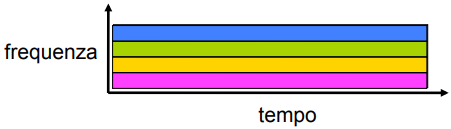
\includegraphics[width=\textwidth]{pic/fdm.png}
                              \label{Divisione di Frequenza}
                          \end{figure}
                    \item \textbf{Divisione di Tempo}
                          \begin{figure}[H]
                              \centering
                              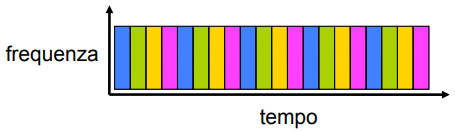
\includegraphics[width=\textwidth]{pic/tdm.png}
                              \label{Divisione di Tempo}
                          \end{figure}
                \end{itemize}
                Tutti gli esempi precedenti vengono proposti prendendo in considerazione una situazione con 4 utenti 

            \subsubsection{Commutazione di Pacchetto}
                In questa metodologia il flusso dei dati viene suddiviso in "\textit{pacchetti}" e ciascuno di questi utilizza completamente il canale.\\
                In questo caso non vi è, però, un accesso esclusivo alle risorse o ad una loro parte, infatti i vari pacchetti devono \textit{competere} per per l'accesso ad esse. Le risorse vengono utilizzate infatti a seconda delle necessità risolvendo il problema dell'inattività della Commutazione di Circuito.\\
                Si presti attenzione al fatto che la richiesta di risorse può eccedere il quantitativo di risorse disponibili creando il fenomeno conosciuto come \textbf{congestione}. Nello specifico i pacchetti sia accodano nell'attesa di utilizzare il collegamento, tenendo presente che verranno trasmessi solo dopo che il commutatore avrà ricevuto l'intero pacchetto (\textbf{Store and Forward}).\\
                La Commutazione di Pacchetto permette il \textit{Multiplexing Statistico}.\\
                \\
                Può succedere, a causa dell'impossibilità del buffer di fare lo storage di altri pacchetti, che alcuni di questi vengano scartati. Quando un pacchetto viene scartato può essere ritrasmesso come no.\\
                \\
                L'arrivo dei pacchetti può avvenire in ritardo, distinguiamo 4 tipi di ritardo
                \begin{itemize}
                    \item \textbf{Ritardo di Elaborazione del Nodo}
                    \item \textbf{Ritardo di Accodamento}
                    \item \textbf{Ritardo di Trasmissione}
                    \item \textbf{Ritardo di Propagazione}
                \end{itemize}

                \subsubsubsection{Ritardo di Elaborazione del Nodo}
                    Può essere causato dal controllo degli errori sul bit o dalla determinazione del canale di uscita

                \subsubsubsection{Ritardo di Accodamento}
                    Può essere causato dall'attesa di trasmissione o da un eccessiva congestione del router

                \subsubsubsection{Ritardo di Trasmissione}
                    Si calcola come \textit{L/R}, con R=\textit{Frequenza di trasmissione del collegamento (in bps)} e L= \textit{Lunghezza del pacchetto}

                \subsubsubsection{Ritardo di Propagazione}
                    Si calcola come \textit{d/s}, con d= \textit{Lunghezza del collegamento fisico} e s= \textit{Velocità di propagazione del collegamento}

\newpage                    
    \section{Il Modello a Strati}
        La problematica legata alla comunicazione tra sistemi è costituita da due sottoproblemi
        \begin{enumerate}
            \item Il linguaggio utilizzato
            \item La modalità di trasmissione delle informazioni
        \end{enumerate}               
        Creiamo quindi un modello che descriva le caratteristiche della comunicazione. In questo chiameremo il linguaggio come \textbf{Comunicazione Logica} ed le modalità di scambio come \textbf{Cominicazione Fisica}.\\
        Con il fine di semplificare il tutto, viene adottato un approccio a strati basato sul "\textit{divide et impera}". Vi sono però delle regole
        \begin{itemize}
            \item Ogni livello comunica solo con i due livelli \textit{adiacenti}. Riceve il messaggio da quello superiore, lo elabora e lo spedisce al livello inferiore (Comunicazione Fisica)
            \item Il messaggio viene rimandato con informazioni aggiuntive rispetto a quando viene ricevuto, grazie all'attività di elaborazione
            \item Ogni livello colloquia con il suo omologo di una altra macchina (Comunicazione Logica) 
        \end{itemize}
        Tra ogni coppia di livelli adiacenti esiste un \textbf{interfaccia} che definisce i \textit{servizi} offerti dal livello sottostante a quello superiore. Per espletare i suoi servizi, ogni livello compie una serie di funzioni che verranno poi sfruttate attraverso richieste (\textit{primitive}).\\
        Queste primitive possono essere di 4 tipi
        \begin{itemize}
            \item \textbf{Request}: Richiesta di un servizio
            \item \textbf{Indication}: Indicazione di un evento
            \item \textbf{Response}: Risposta ad un indicazione
            \item \textbf{Confirm}: Conferma di una richiesta 
        \end{itemize}
        Per ogni \textit{Request} esiste un \textit{Indication} di entità pari.\\
        \\
        Abbiamo invece due tipi di \textbf{servizi}
        \begin{itemize}
            \item \textbf{Connection Oriented}: Simulano una connessione punto-punto (gestiscono consegna sequenziale)
            \item \textbf{Connectionless}: Semplice passaggio dell'informazione senza preoccuparsi si instaurare una connessione
        \end{itemize} 
        Per ogni tipo di servizio è possibile associare una \textbf{Quality of Service}
        \begin{itemize}
            \item \underline{Affidabile}: Non ci sono perdite perchè il ricevente informa sempre dell'avvenuta ricezione
            \item \underline{Non Affidabile}: Sono possibili perdite di dati
        \end{itemize}

    \section{Livello Applicazione}
        \subsection{Architettura Client-Server}
            \paragraph{Server} Il \textit{server} è un host sempre attivo con indirizzo IP fisso.
            \paragraph{Client} Il \textit{client} comunica con il server in qualunque momento esso voglia, può avere indirizzo IP dinamico. Non comunica direttamente con gli altri client.

            Sugli host vengono eseguiti dei programmi, detti \textbf{processi}, che comunicano tra di loro utilizzando \textit{schemi interprocesso} definiti dal Sistema Operativo. Processi su host differenti comunicano attraverso \textit{messaggi}.\\
            Distinguiamo due tipologie di processi
            \begin{itemize}
                \item \textbf{Processi Client}: Processo che da inizio alla comunicazione
                \item \textbf{Processi Server}: Processo che attende di essere contattato
            \end{itemize}

            \paragraph{Socket} Un processo invia e riceve messaggi tramite la sua \textit{Socket}. Il concetto è analogo a quello di \textit{porta}
            Un processo che vuole inviare un messaggio lo fa uscire dalla propria socket. Questo presuppone l'esistenza di un'infrastruttura esterna che trasporterà il messaggio attraverso la rete fino alla porta del processo di destinazione.\\
            Notare il fatto che non basti essere a conoscenza dell'IP della destinazione, sullo stesso host possono girare più processi, è per questo importante indicare anche la porta associata al processo in questione.

        \subsection{Servizi dei protocolli di trasporto Internet}
            \subsubsection{Servizio di TCP}
                \begin{itemize}
                    \item \underline{Connection oriented}: Richiede un setup tra i processi client e server
                    \item \underline{Controllo di Flusso}: il mittente non vuole sovraccaricare il destinatario
                    \item \underline{Controllo della Congestione}: Riduce il processo di invio quando la rete è sovraccaricata
                    \item \underline{NON OFFRE}: Temporizzazione, garanzia su ampiezza di banda minima, sicurezza 
                \end{itemize}

            \subsubsection{Servizio di UDP}
                \begin{itemize}
                    \item Trasferimento dati inaffidabile tra processi d'invio e di ricezione
                    \item \underline{NON OFFRE}: Setup della connessione, affidabilità, controllo di flusso, controllo di congestione, temporizzazione, ampiezza di banda minima e sicurezza
                \end{itemize}

        \subsection{Web e HTTP}
            Una pagina web è costituita da oggetti, questi possono essere varie cose, come immagini, filmati, file HTML, ecc.\\
            Ogni pagina web è formata da un file HTML di base che include i diversi oggetti referenziati da un \textbf{URL}.\\
            \\
            Il protocollo che gestisce le applicazioni web è l'\textbf{HTTP (HyperText Transfer Protocol)} e si basa sul modello \textit{client/server}
            \begin{itemize}
                \item Il \textit{client} richiede, riceve e "visualizza" gli oggetti web
                \item Il \textit{server} invia questi oggetti in risposta ad una richiesta
            \end{itemize}
            Questo protocollo usa \textit{TCP}, prima il client instaura una connessione TCP (ovvero crea una \textit{socket}) con il server (\textit{Porta 80}), il server accetta la connessione TCP dal client in modo da poter cominciare lo scambio tra i due, alla fine la connessione viene chiusa.\\
            HTTP è un protocollo \textbf{stateless}, ovvero il \textit{server} non tiene traccia delle richieste del client.\\
            Posso avere 2 tipi di connessioni HTTP
            \begin{itemize}
                \item \textbf{Connessioni non persistenti}: Almeno un oggetto viene trasmesso su una connessione TCP
                \item \textbf{Connessioni persistenti}: Più oggetti possono essere trasmessi su una singola connessione TCP
            \end{itemize} 

            \subsubsection{Connessioni non persistenti}
                Dopo che l'utente ha inserito l'URL
                \begin{enumerate}
                    \item Il client HTTP comincia una connessione TCP con il server HTTP sulla porta 80
                    \item Il server HTTP, in attesa di una connessione TCP alla porta 80 "accetta" la connessione e avvisa il client
                    \item Il client trasmette un \textit{messaggio di richiesta} nella socket della connessione TCP indicando quale oggetto vuole
                    \item Il server HTTP riceve il messaggio di richiesta, forma un messaggio di risposta che contiene l'oggetto richiesto, lo invia poi nella sua socket
                    \item Il server HTTP chiude la connessione TCP
                    \item Il client HTTP riceve il messaggio contenente la risposta, esaminando poi il file HTML ripeterà $ n $ volte questi passi per ogni oggetto aggiuntivo che gli servirà
                \end{enumerate}
                In base a quanto appena visto definiamo ora il concetto di \textbf{Round Trip Time (RTT)}, ossia il tempo di risposta. Esso viene indicato come il tempo che ci mette un pacchetto per andare da client al server HTTP e ritornare.\\
                Tenuto conto che ci dovrà essere un pacchetto per iniziare la connessione, una richiesta e l'effettivo trasferimento dei dati, è intuitivo dire che in totale ci vorrà un tempo di \textit{2RTT + tempo di trasmissione}.

            \subsubsection{Connessioni persistenti}
                In questo caso il server lascia la connessione aperta dopo l'invio di una risposta in modo che i successivi messaggi tra client e server HTTP sfrutteranno questa connessione già esistente. Il client invia le richieste non appena incontra un oggetto referenziato nel file HTML principale, mettendoci un RTT per tutti gli oggetti

            \subsubsection{Messaggi HTTP}
                Si possono avere 2 tipi di messaggi
                \begin{itemize}
                    \item Messaggi di \textbf{Richiesta}
                    \item Messaggi di \textbf{Risposta}
                \end{itemize}

                \subsubsubsection{Messaggi di Richiesta}
                \begin{figure}[H]
                    \centering
                    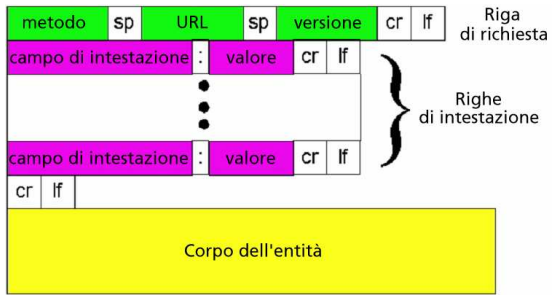
\includegraphics[width=\textwidth]{pic/richiesta_http.png}
                    \label{Messaggi di RIchiesta HTTP}
                \end{figure}
                Per eseguire \textit{l'upload dell'input di un form} posso usare due metodi
                \begin{itemize}
                    \item \textbf{Metodo Post}: La pagina web spesso include form per input dall'utente, questo input viene incorporato nel messaggio al server
                    \item \textbf{Metodo URL}: Usa il metodo \textit{GET}, l'input arriva nel campo URL
                \end{itemize}
                Definiamo quindi i tipi di metodi
                \begin{itemize}
                    \item \textbf{HTTP/1.0}
                          \begin{itemize}
                              \item GET
                              \item POST
                              \item HEAD (Esclusione di un oggetto nella  risposta)
                          \end{itemize}
                    \item \textbf{HTTP/1.1}
                          \begin{itemize}
                              \item GET, POST, HEAD (Come 1.0)
                              \item PUT (Include il file nel corpo dell'oggetto e lo invia al percorso specificato nell'URL)
                              \item DELETE (Cancella il file specificato nell'URL)
                          \end{itemize}
                \end{itemize}

                \subsubsubsection{Messaggi di Risposta}
                    Il formato della risposta HTTP è molto simile a quello della richiesta, vengono introdotti dei codici di stato nella prima riga. Questi possono avere vari significati.
                    \begin{itemize}
                        \item \textbf{200 OK}: La richiesta ha avuto successo
                        \item \textbf{301 Mooved Permanently}: Oggetto trasferito, nuova posizione nel campo \textit{Location} della risposta
                        \item \textbf{400 Bad Request}: Messaggio non compreso dal server HTTP
                        \item \textbf{404 Not Found}: Il documento richiesto non si trova sul server
                        \item \textbf{500 HTTP Version not Supported}: Il server non ha la versione del protocollo HTTP
                    \end{itemize}

            \subsubsection{Cookie}
                Sono formati da quattro componenti
                \begin{enumerate}
                    \item Riga di intestazione nella risposta HTTP
                    \item Riga di intestazione nella richiesta HTTP
                    \item File mantenuto nel terminale dell'utente e gestito dal browser
                    \item Un database sul sito
                \end{enumerate}
                Ma cosa possono contenere i cookie? Nello specifico
                \begin{itemize}
                    \item Autorizzazione
                    \item Carta per Acquisti
                    \item Raccomandazioni
                    \item Stato della Sessione (E-Mail)
                \end{itemize}

            \subsubsection{Cache Web}
                L'obiettivo è quello di soddisfare la richiesta dell'utente senza contattare il server d'origine. In questo modo il browser invia tutte le richieste HTTP al \textit{Server Proxy}. Se l'oggetto richiesto è nella cache allora viene ritornato, altrimenti il server proxy si fa carico della richiesta al server d'origine, ritornando poi l'oggetto al client.
                Questo metodo è stato implementato al fine di rendere più veloce la risposta del server al client, riducendo di conseguenza il traffico.

                \subsubsubsection{GET Condizionale}
                    L'obiettivo è quello di non inviare un oggetto se la \textit{cache} ne ha già una copia aggiornata. Nella \textit{richiesta} viene specificata la data di ultima modifica dell'oggetto, se la copia cache è aggiornata il server non invia l'oggetto nella risposta.
                
        \subsection{FTP}
            Il \textbf{File Transfer Protocol} serve per il trasferimento di file da/a un host remoto.\\
            Il \textit{client} è il lato che inizia il trasferimento, il \textit{server} è un host remoto. Utilizza la \textit{porta 21}.\\
            \\
            Il client FTP contatta il server alla porta 21, specificando TCP come protocollo di trasporto. Il client ottiene l'autorizzazione sulla connessione di controllo, tramite comandi su questa cambia poi la \textit{directory remota}.\\
            Quando il server riceve un comando per trasferire un file viene aperta una connessione TCP verso il client, questa verrà poi chiusa alla fine del trasferimento.\\
            \\
            Ecco una lista di \textit{comandi}
            \begin{itemize}
                \item \textbf{USER username}
                \item \textbf{PASS password}
                \item \textbf{LIST}: Elenca i file della directory
                \item \textbf{RETR filename}: GET su un file della directory
                \item \textbf{STOR filename}: PUT su un file della directory
            \end{itemize}
            E \textit{risposte} comuni
            \begin{itemize}
                \item \textbf{331 username OK, password required}
                \item \textbf{125 data connection already open; transfer starting}
                \item \textbf{425 Can't open data connection}
                \item \textbf{452 Error writing file}
            \end{itemize}   

        \subsection{Posta Elettronica}
            Vi sono 3 requisiti fondamentali per l'utilizzo della \textit{Posta Elettronica}, il primo, banalmente, è un utente, servono poi un server di posta e \textbf{SMTP (Simple Mail Transfer Protocol)}.\\
            Penso sia scontato spiegare quale sia il ruolo dell'utente, passiamo dunque al server di posta. Ogni mail server è composto da una \textit{casella di posta (mailbox)} che contiene i messaggi in arrivo. Abbiamo poi una \textit{coda di messaggi} da trasmettere e il protocollo SMTP che gestisce l'invio dei messaggi da un server di posta all'altro.
            
            \subsubsection{SMTP}
                Il \textit{Simple Mail Transfer Protocol} usa TCP per inviare messaggi dal client al server, \textit{porta 25}. Il trasferimento avviene in modo diretto tra due server, questo avviene in 3 fasi
                \begin{itemize}
                    \item \textit{Handshaking}
                    \item \textit{Trasferimento del messaggio}
                    \item \textit{Chiusura} 
                \end{itemize}
                Alcuni dettagli da ricordare sono che SMTP usa una connessione persistente ed il messaggio sia nel formato \textit{ASCII a 7 bit}.\\
                Possiamo paragonare SMTP e HTTP molto facilmente, infatti se HTTP esegue un azione di \textit{pull} SMTP ne esegue un di \textit{push}, la differenza sta nel come vengono inviati gli oggetti. HTTP incapsula ogni oggetto in un proprio messaggio di risposta mentre SMTP può inviare più oggetti in un singolo messaggio.\\
                \\
                I messaggi hanno un proprio formato, naturalmente, sono infatti composti da \textit{intestazione} e \textit{corpo}. L'intestazione contiene \textit{from}, \textit{to} e \textit{subject}, banale capire cosa sono, mentre il corpo è l'effettivo messaggio. Si può invece usare \textbf{MIME} per estendere il messaggio. Con questo viene aggiunto il supporto a
                \begin{itemize}
                    \item L'impiego di codifiche diverse da \textit{ASCII}
                    \item L'aggregazione di messaggi
                    \item La codifica di messaggi (o di una loro parte) non testuali
                \end{itemize}

            \subsubsection{Protocolli di Accesso}
                Tra questi troviamo
                \begin{itemize}
                    \item \textbf{POP3}: Autorizzazione tra utente e server e download
                    \item \textbf{IMAP}: Manipolazione di messaggi
                    \item \textbf{HTTP}
                \end{itemize}

                \subsubsubsection{POP3}
                    Fase di Autorizzazione
                    \begin{itemize}
                        \item \textit{Comandi lato client}
                              \begin{itemize}
                                  \item \textbf{user}: Dichiara il nome utente
                                  \item \textbf{pass}: Password 
                              \end{itemize}
                        \item \textit{Risposte del server}
                              \begin{itemize}
                                  \item \textbf{+OK}
                                  \item \textbf{-ERR}
                              \end{itemize}
                    \end{itemize}
                    Nelle transazione (lato client)
                    \begin{itemize}
                        \item \textbf{list}: Elenca i numeri dei messaggi
                        \item \textbf{retr}: Ritorna i messaggi in base al numero
                        \item \textbf{dele}: Cancella un messaggio
                        \item \textbf{quit}
                    \end{itemize}
                    POP3 è un protocollo stateless tra le varie sessioni

                \subsubsubsection{IMAP}
                    Con \textit{IMAP} i messaggi vengono mantenuti sul server, offrendo inoltre la possibilità di organizzarli in cartelle. A differenza di POP3 lo stato dell'utente viene mantenuto tra le varie sessioni. 

                \subsubsubsection{HTTP}
                    Alcuni server di posta utilizzano \textit{HTTP} per l'interazione con i messaggi di posta in entrata, tra questi \textit{Gmail, Yahoo! Mail} e \textit{Hotmail} per citarne alcuni.

        \subsection{DNS}
            Le persone come noi hanno molti modi per identificarsi, come il Nome o il Codice Fiscale. Gli Host (o i Router) invece vengono tanto identificati con un codice a \textit{32 bit} detto \textit{Indirizzo IP} quanto da un nome, si pensi al fatto che per connettersi a \textit{Google} non si digita un IP ma \textit{www.google.it}.\\
            Per l'associazione tra nome e IP si una il \textbf{DNS (Domain Name System)}. DNS è un \textit{database distribuito}, implementato come dei \textit{server DNS} che si rapportano l'uno con l'altro gerarchicamente.\\
            \begin{figure}[H]
                \centering
                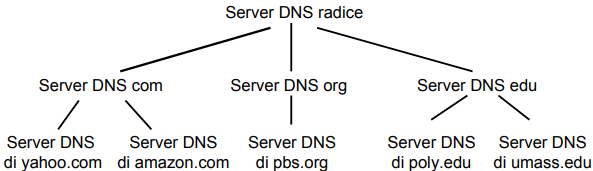
\includegraphics[width=\textwidth]{pic/gerarchia_dns.png}
                \label{Gerarchia dei Server DNS}
            \end{figure}
            Il server \textit{Radice} viene contattato da un server DNS locale che non può risolvere un nome, se anch'esso non conosce la mappatura contatta un server DNS autorizzato, ottenendola. La ritorna poi al server DNS locale.

            \subsubsection{Server TLD}
                I \textbf{Top-Level Domain} si occupano dei nomi \textit{com, org, edu, ecc}. e tutti quelli locali di alto livello (\textit{uk, fr, ecc.}).\\
                Ogni organizzazione dotata di host Internet pubblici deve fornire i record DNS che mappano i nomi di tali host agli indirizzi IP. 

            \subsubsection{Server DNS Locali}
                Non appartengono strettamente alla gerarchia dei server, ogni ISP ne ha uno. Quando un host fa una richiesta DNS questa viene inviata al suo server DNS locale (che farà da proxy inoltrandola alla gerarchia di server DNS)

            \subsubsection{Caching e aggiornamento dei record}
                Quando un server apprende una mappatura la mette in \textit{cache}, dove però quest'informazione sparisce dopo un certo periodo di tempo. Tipicamente, un server DNS locale memorizza nella cache gli IP dei server TLD

                \subsubsubsection{Record DNS}
                    Il formato dei \textbf{Record di Risorsa (RR)} è il seguente: \textit{(name, value, type, tll)}
                    \begin{itemize}
                        \item \textbf{Type=A}: \textit{name} è il nome dell'host mentre \textit{value} è l'indirizzo IP
                        \item \textbf{Type=NS}: \textit{name} è il dominio (\underline{Esempio}: .com) e \textit{value} è il nome dell'host del server di competenza
                        \item \textbf{Type= CNAME}: \textit{name} è l'alias di qualche nome canonico (\textit{www.ibm.com} è in realtà \textit{servereast.backup2.ibm.com}). \textit{value} è il nome canonico
                        \item \textbf{Type=MX}: \textit{value} è il nome del server di posta associato a \textit{name}
                    \end{itemize}

                \subsubsubsection{Messaggio DNS}
                    Le domande (\textit{query}) ed i messaggi di risposta condividono lo stesso formato
                    \begin{figure}[H]
                        \centering
                        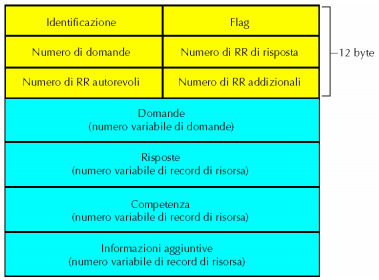
\includegraphics[width=\textwidth]{pic/messaggio_dns.png}
                        \label{}
                    \end{figure} 
                    Dove
                    \begin{itemize}
                        \item \textbf{Identificazione}: Numero di \textit{16 bit} per la domanda, la risposta usa lo stesso numero
                        \item \textbf{Flag}:
                              \begin{itemize}
                                  \item Domanda o risposta
                                  \item Richiesta di ricorsione
                                  \item Ricorsione disponibile
                                  \item Risposta di competenza
                              \end{itemize}
                    \end{itemize}
        
        \subsection{Programmazione delle Socket}
            La socket è \textit{l'interfaccia} di un host locale, creata dalle applicazioni e gestita dal Sistema Operativo. Su questa il processo di un applicazione può inviare e ricevere messaggi al/dal processo di un altra applicazione. Più semplicemente è il punto in cui un processo accede al canale di comunicazione attraverso una porta.\\
            La \textbf{Socket API}, introdotta nel 1981 sfrutta il paradigma client/server. Vi sono fondamentalmente due tipi di servizio tramite Socket API
            \begin{itemize}
                \item Datagram Socket (\textit{utilizza UDP}, inaffidabile)
                \item Stream Socket (\textit{utilizza TCP}, affidabile e orientata ai Byte)
            \end{itemize} 

            \subsubsection{Programmazione con TCP}
                Il client, per prima cosa deve contattare il server e quest'ultimo deve essere in esecuzione ed aver creato uuna socket che da il "benvenuto" al client.\\
                Il client, a sua volta, per contattare il server crea una socket TCP specificando IP e numero di porta del processo server. Creata questa il client TCP stabilisce al connessione con il server.\\
                Al momento del contatto da parte del client il server crea la socket per il suo processo, permettendo così la comunicazione con il processo client. È possibile quindi che lo stesso server comunichi con più client contemporaneamente.\\
                Passiamo ora d un po' di terminologia
                \begin{itemize}
                    \item \textbf{Flusso (Strem)}: Sequenza di caratteri che fluisce da/verso un processo
                          \begin{itemize}
                              \item \textbf{Flusso d'Ingresso (Input Stream)}: Collegato ad un origine d'ingresso (tastiera o socket, per esempio)
                              \item \textbf{Flusso d'Uscita (Output Stream)}: Collegato ad un uscita per il processo (monitor o socket ad esempio)
                          \end{itemize} 
                \end{itemize}

            \subsubsection{Programmazione con UDP}
                Essendo gestita tramite UDP non vi è una "connessione" tra client e server. Manca infatti la fase di \textit{handshaking}. Per l'invio di ogni pacchetto viene allegatala porta di destinazione e l'IP del destinatario.\\
                Il server dovrà quindi estrarre IP e porta direttamente dal pacchetto arrivatogli. I pacchetti possono andare persi oppure arrivare in ordine diverso rispetto a quello di invio. 

\newpage                
    \section{Livello di Trasporto}
        Il \textbf{Livello di Trasporto} si occupa di fornire un canale end-to-end ideale e privo di errori. Come tutti i livelli offre dei servizi al livello superiore e esegue delle funzioni.\\
        Fornisce essenzialmente due servizi
        \begin{itemize}
            \item \textbf{Connection-oriented affidabile}: TCP
            \item \textbf{Connectionless non affidabile}: UDP
        \end{itemize}
        Le funzioni svolte sono
        \begin{itemize}
            \item Indirizzamento a livello applicazione, multiplexing e demultiplexing
                  \begin{itemize}
                      \item Differenziazione delle diverse applicazioni che utilizzano il protocollo per il trasferimento dati
                      \item multiplazione in caso di reti comuni
                  \end{itemize}
            \item Instaurazione e gestione delle connessioni
            \item Recupero degli errori
            \item Consegna ordinata dei segmenti
            \item Controllo di flusso
            \item Controllo della congestione
        \end{itemize}
        È importante ricordare che tutti questi servizi sono serviti da \textit{TCP} ma solo il primo viene offerto a \textit{UDP}

        \subsection{TCP}
            Il \textbf{TCP (Transmission Control Protocol)} si occupa del controllo di trasmissione rendendo \textit{affidabile} la comunicazione tra mittente e destinatario.

            \subsubsection{Header TCP}
                \begin{figure}[H]
                    \centering
                    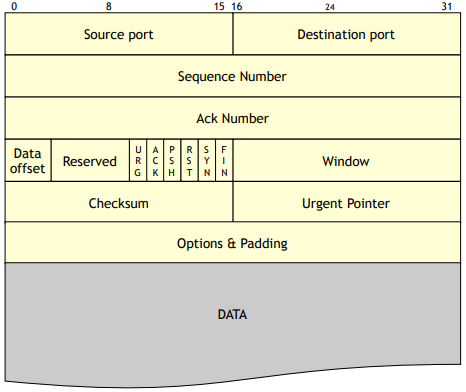
\includegraphics[width=\textwidth]{pic/header_tcp.png}
                    \label{Header TCP}
                \end{figure}
                \begin{itemize}
                    \item \textbf{Source/Destinazion Port} (16 bit ciascuna)\\ 
                          Indirizzi della porta sorgente e destinazione (rispettivamente)
                    \item \textbf{Sequence Number} (32 bit)\\
                          Numero di sequenza del primo byte del payload (DATA nell'immagine)
                    \item \textbf{Acknowledge Number} (32 bit)\\
                          Numero di sequenza del prossimo byte che si intende ricevere (solo se questo segmento è \textit{ACK})
                    \item \textbf{Offset} (4 bit)\\
                          Lunghezza dell'header, in multipli di 32
                    \item \textbf{Resereved} (6 bit)\\
                          Riservato per usi futuri
                    \item \textbf{Window} (16 bit)\\
                          Ampiezza della \textit{Reciving Window} (solo se questo segmento è \textit{ACK})
                    \item \textbf{Checksum} (16 bit)\\
                          Risultato di un calcolo che serve per comprendere se il segmento contiene errori
                    \item \textbf{Urgent Pointer} (16 bit)\\
                          Indica che il ricevente deve iniziare a leggere il campo DATA dal numero di byte specificato. usato se si inviano comando che generano eventi \textit{asincroni} urgenti
                \end{itemize}
                Vi sono anche 6 \textbf{flag}
                \begin{itemize}
                    \item \textbf{URG}: 1 se urgente, in questo caso \textit{Urgent Pointer} ha significato
                    \item \textbf{ACK}: 1 se ACK, in questo caso \textit{Acknowledge Number} è un numero valido
                    \item \textbf{PSH}: 1 se il trasmettitore usa il comando \textit{PUSH}
                    \item \textbf{RST}: Reset della connessione senza chiusura esplicita
                    \item \textbf{SYN}: Utilizzato durante il setup della connessione per comunicare il numero di sequenza iniziale (\textit{ISN})
                    \item \textbf{FIN}: Usato per chiusura esplicita della connessione
                \end{itemize}
                
            \subsubsection{Indirizzamento}
                Come posso distinguere diverse applicazioni al livello di trasporto? Si utilizzano le \textbf{porte}, ossia un codice che identifica un'applicazione. Conoscendo questo ora è possibile definire le \textit{socket} come tuple che identificano la connessione tra due applicazioni.
                Il numero di porta può essere
                \begin{itemize}
                    \item \textbf{Statico (Porte Note)}: Identificativo ad applicazioni largamente utilizzati. Sono stabilite dall'\textbf{IANA} (\textit{Internet Assigned
                    Number Authority}) e sono quelle inferiori al 1024
                    \item \textbf{Dinamico}: Identificativi assegnati direttamente dal Sistema Operativo al momento dell'apertura della connessione  
                \end{itemize}
                L'utilizzo delle porte, insieme agli indirizzi IP sorgente e destinazione (\textit{socket} quindi) servono per multiplexing/demultiplexing dati da parte di TCP. I socket identificano univocamente una connessione (su cui passa un unico flusso di informazioni).

            \subsubsection{Gestione delle connessioni}
                \subsubsubsection{Instaurazione della Connessione}
                    Il TCP è un protocollo \textit{connection-oriented}, ossia ci deve essere una connessione tra mittente e destinatario prima di inviare dati.\\
                    Quest'instaurazione avviene attraverso un \textbf{Three-Way Handshake}
                    \begin{itemize}
                        \item La stazione A (richiedente della connessione) invia il segmento di SYN specificando
                              \begin{itemize}
                                  \item Numero di porta dell'applicazione cui si vuole accedere
                                  \item ISN (Initial Sequence Number)
                              \end{itemize}
                        \item La stazione B (ricevente della richiesta di connessione) risponde con un segmento SYN specificando
                              \begin{itemize}
                                  \item ISN
                                  \item ACK al segmento SYN di A
                              \end{itemize}
                        \item La stazione A riscontra il segmento SYN di B con un ACK
                    \end{itemize}
                    Questa procedura apre due canali monodirezionali, che visti come un'unica entità risultano un unico canale monodirezionale.\\
                    I segmenti SYN, ACK, dati, ecc. sono particolari, i loro campi dell'header assumono valori particolari
                    \begin{itemize}
                        \item Un segmento SYN è un segmento vuoto, possiede solo l'header ed il suo flag \textit{SYN} è posto a 1
                        \item Un segmento ACK e un segmento vuoto, possiede solo l'header ed il suo flag \textit{ACK} è posto a 1
                        \item Un segmento SYN ACK e un segmento vuoto, possiede solo l'header ed il suoi flag \textit{SYN} e \textit{ACK} sono posti a 1
                        \item Un segmento dati è un segmento contiene i dati dell'applicazione in cui i falg \textit{SYN} e \textit{ACK} sono a 0 
                    \end{itemize}

                    \paragraph{MSS (Maximum Segment Size)}
                        Nel campo \textbf{Options \& Padding} dell'header è possibile inserire l'MSS, questo esprime la dimensione massima del campo dati dei segmenti che verranno inviati (in Byte, default 536 Byte)

                \subsubsubsection{Terminazione della Connessione}
                    Procedura di terminazione
                    \begin{itemize}
                        \item La stazione che non ha più dati da trasmettere e vuole terminare la connessione invia un segmento FIN
                        \item La stazione che riceve il segmento FIN riscontra questo con un ACK e indica all'applicazione che la connessione entrante è stata chiusa
                    \end{itemize}
                    Se il processo di chiusura termina in questo modo siamo davanti ad una chiusura parziale della comunicazione (si parla di \textit{half-close}). Nell'altro verso la comunicazione può continuare, per chiudere completamente la connessione anche l'altra stazione deve eseguire l'half-close.    

            \subsubsection{Gestione di Errori e Perdite}
                Il TCP è un protocollo \textbf{affidabile}, garantisce infatti la corretta ed ordinata consegna dei segmenti.\\
                Deve quindi poter gestire
                \begin{itemize}
                    \item Gli errori (individuati tramite \textit{Checksum})
                    \item Perdita di segmenti (individuata tramite gli ACK, se non avviene il riscontro di un segmento questo viene considerato perso)
                \end{itemize}
                Nel caso in cui ci si trovi in una di queste due situazioni TCP ritrasmette i segmenti. Questa tecnica prende il nome di "\textit{"positive acknowledgement with retransmission"}.\\
                Nella versione base di questa tecnica, la sorgente non ritrasmette il segmento successivo fino al riscontro di quello correntemente inviato.\\
                \\
                Ma per quanto devo aspettare prima di considerare un segmento perso? Viene quindi introdotto il concetto di \textbf{RTO (Retransmission Timeout)}. Come si può facilmente immaginare, indica la quantità di tempo entro la quale la sorgente si aspetta di ricevere un ACK prima di considerare il segmento perso.\\
                Naturalmente questo non è un valore statico, viene bensì ricalcolato di volta in volta, per primo durante l'instaurazione della connessione, poi durante la trasmissione dei dati. Questo calcolo si basa sull'\textbf{RTT (Round Trip Time)} (tempo tra l'invio di un pacchetto ed il suo riscontro) 

                \subsubsubsection{Stima dell'RTT}
                    Il calcolo è molto semplice
                    \[
                        SRTT = (\alpha*SRTT_{precedente})+((1-\alpha)*RTT_{istantaneo})    
                    \]
                    con $ \alpha \in [0,1] $.\\
                    Il valore di $ \alpha $ indica
                    \begin{itemize}
                        \item Stabilità, SRTT non viene influenzato da singoli segmenti aventi RTT molto diversi ($ \alpha = 1 $)
                        \item Instabilità, SRTT dipende molto dalla misura puntuale dei singoli RTT istantanei
                    \end{itemize}

                \subsubsubsection{Stime dell'RTO}
                    \[
                        RTO = \beta*SRTT    
                    \]
                    con $ \beta $ tipicamente 2 (\textit{Delay Variance Factor})\\
                    In caso di ritrasmissione, l'RTO viene ricalcolato in base ad un processo di \textit{exponential backoff}.\\
                    Infatti se è scaduto l'RTO molto probabilmente c'è congestione
                    \[
                        RTO_{new} = 2RTO 
                    \]

            \subsubsection{Controllo di Flusso}
                Anche se possono sembrare due concetti coincidenti, \textit{Controllo di Flusso} e \textit{Controllo di Congestione} esprimono cose diverse
                \begin{itemize}
                    \item \textbf{Controllo di Flusso}: È un'azione preventiva finalizzata a limitare l'immissione di dati in base alla capacità della rete
                    \item \textbf{Controllo di Congestione}: Reazione all'eccessiva congestione della rete
                \end{itemize}
                Con la tecnica di postive acknoledgement with retransmission abbiamo visto che una stazione invia un nuovo segmento solo se l’ultimo è stato riscontrato, questa tecnica è di suo un azione di \textit{Controllo di Flusso}, anche se poco efficiente.

                \subsubsubsection{Controllo di Flusso a Finestra}
                    Per aumentare l'efficienza è possibile trasmettere più segmenti consecutivi senza attendere ogni singolo riscontro. Alla ricezione dei riscontri dei segmenti iniziali della sequenza, la finestra scorre a destra permettendo la trasmissione dei nuovi segmenti. Questa tecnica è detta della \textbf{Sliding Window}.\\
                    Consideriamo ora di avere una finestra di dimensione troppo piccola, in questo caso vi è un sottoutilizzo della banda. Al contrario invece, se la finestra è troppo grande i riscontri potrebbero arrivare prima che tutti i segmenti vengano inviati.\\     
                    \\
                    Come comportarsi invece in caso di perdita di segmenti? Abbiamo detto che, in caso di perdita, passato un RTO la sorgente provvede a reinviarlo. E se il segmento facesse parte di una finestra (multipli pacchetti inviati)?\\
                    Possibili soluzioni
                    \begin{itemize}
                        \item \textbf{Go-back-N}: La finestra torna indietro e vengono ritrasmessi tutti i segmenti
                        \item \textbf{Selective Repeat}: Viene ritrasmesso solo il segmento perso
                    \end{itemize}

            \subsubsection{Controllo di Congestione}
                A causa di un eccessiva congestione della rete alcuni segmenti potrebbero venire persi, la sorgente quindi dovrebbe diminuire il tasso di immissione dei nuovi segmenti. Questo è detto \textbf{Controllo di Congestione}

                \subsubsubsection{Congestion Window}
                    In caso di congestione il controllo di flusso a finestra protegge implicitamente anche la rete, tuttavia questo potrebbe non essere sufficiente. Difatti va ancora stabilita la dimensione ottimale della finestra.\\
                    La soluzione sta nello stabilire dinamicamente la dimensione della finestra, questa prende quindi il nome di \textbf{Congestion Window (CWND)}.

                \subsubsubsection{Algoritmi per il controllo di congestione}
                    Esistono due algoritmi che regolano la dimensione della CWND
                    \begin{itemize}
                        \item \textbf{Slow Start}: Per ciascun riscontro ricevuto la CWND aumenta di dimensione, quindi la CWND ha un andamento esponenziale
                        \item \textbf{Congestion Avoidance}: Per ciascun riscontro ricevuto la CWND aumenta di 1/CWND, quindi la CWND ha un andamento lineare
                    \end{itemize}
                    Ci sono alcune variabili da tenere in considerazione
                    \begin{itemize}
                        \item \textbf{CWND}: Dimensione della finestra di trasmissione
                        \item \textbf{RECWND (Recieve Window)}: Dimensione della finestra di ricezione, limite massimo della CWND (annunciata dalla \textit{destinazione})
                        \item \textbf{SSTHRESH (Slow Start Threshold)}: Dimensione della CWND raggiunta la quale avviene il passaggio da \textit{Slow Start} a \textit{Congestion Avoidance}
                        \item \textbf{RTT}: Tempo trascorso tra l'invio di un segmento e la ricezione del riscontro
                        \item \textbf{RTO}: Tempo atteso dalla sorgente prima di ritrasmettere un pacchetto di cui non ha ricevuto riscontro 
                    \end{itemize}
                    L'algoritmo che regola la CWND è il seguente
                    \begin{itemize}
                        \item All'inizio della trasmissione si pone
                              \begin{itemize}
                                  \item CWND = 1 segmento
                                  \item SSTHRESH = RECWND o RECWND/2
                              \end{itemize}
                        \item La CWND evolve con \textit{Slow Start} fino a SSTHRESH
                        \item Raggiunto SSTHRESH si passa a \textit{Congestion Avoidance}
                        \item La CWND cresce fino a RECWND
                    \end{itemize}
                    Cosa fare nel caso vi sia perdita di pacchetti o errori? La finestra non si muove e si aspetta RTO, allo scadere del quale si pone
                    \begin{itemize}
                        \item SSTHRESH = CWND/2
                        \item CWND = 1
                    \end{itemize}
                    Si riprende quindi a trasmettere con la tecnica \textit{Go-Back-N}, si prosegue quindi come illustrato prima.\\
                    Se gli errori/perdite fossero consecutivi? Dal secondo in poi si ricalcola RTO con \textit{Exponential Backoff}, la CWND rimane a 1 ma SSTHRESH viene impostato a 2 segmenti.

                \subsubsubsection{Fast Retransmit - Fast Recovery}
                    I segmenti vanno persi o per congestione o per errori di trasmissione. Invece che utilizzare metodi eccessivi, magari per la perdita di un solo segmento, sono stati implementati due algoritmi
                    \begin{itemize}
                        \item \textbf{Fast Retransmit}: Ritrasmette subito il segmento considerato perso
                        \item \textbf{Fast Recovery}: La CWND non viene chiusa
                    \end{itemize}

                \subsubsubsection{ACK Duplicati}
                    Negli ACK il campo Ack Number contiene il successivo numero di sequenza che ci si aspetta arrivi. Se un segmento arriva fuori sequenza, la destinazione invia un ACK indicando il numero di sequenza del segmento che non e’ ancora arrivato.\\
                    La ricezione di un numero sufficientemente alto di ACK duplicati può essere interpretata come forte di indicazione che e’ avvenuta una perdita.\\
                    \\
                    Se arrivano 3 ACK duplicati
                    \begin{itemize}
                        \item SSTHRESH = CWND/2
                        \item Si usa \textit{Fast Retransmit}
                        \item CWND = SSTHRESH + 3 (\textit{Fast Recovery})
                        \item Per ogni successivo ACK duplicato la CWND aumenta di 1
                    \end{itemize} 
                    Quando la sorgente riceve l’ACK che conferma la ricezione del segmento ritrasmesso
                    \begin{itemize}
                        \item CWND = SSTHRESH
                        \item Si prosegue utilizzando \textit{Congestion Avoidance}
                    \end{itemize}
                    Se il segmento ritrasmesso viene perso, si attende lo scadere del RTO, la CWND torna a 1 e si riparte in Slow Start.\\
                    Se viene perso piu’ di un segmento: l’algoritmo cerca di recuperare il primo, anche se ce la fa, arrivano gli ACK duplicati dei successivi segmenti persi che l’algoritmo non sa trattare, per cui scade il RTO.
                
        \subsection{UDP}
            Il protocollo \textbf{UDP (User Datagram Protocol)} è un protocollo \textit{connectionless non affidabile}. Esso svolge solo funzione di indirizzamento delle porte, infatti non gestisce
            \begin{itemize}
                \item Connessioni
                \item Controllo di Flusso
                \item Recupero errori (li \textit{rileva} e basta)
                \item Controllo della Congestione
                \item Riordinamento dei pacchetti
            \end{itemize}         
            Per tutte queste funzioni si affida ai livelli superiori.
            
            \subsubsection{Header UDP}
                \begin{figure}[H]
                    \centering
                    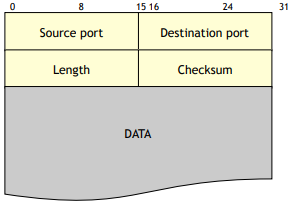
\includegraphics[width=\textwidth]{pic/header_udp.png}
                    \label{Header UDP}
                \end{figure}
                \begin{itemize}
                    \item \textbf{Source/Destination Port} (16 bit)\\
                          Identificano i processi sorgente e destinazione dei dati
                    \item \textbf{Length} (16 bit)\\
                          Lunghezza in Byte, header compreso
                    \item \textbf{Checksum} (16 bit)\\
                          Campo di controllo per il rilevamento errori nel campo DATA
                \end{itemize}

\newpage                
    \section{Livello di Rete}
        La funzione chiave del \textbf{Livello di Rete} è il \textbf{routing}, ovvero la determinazione del percorso che dovranno seguire i datagrammi dalla sorgente alla destinazione. Altra funzione fondamentale è il \textbf{forwarding} che trasferisce i pacchetti da una porta di input ad una porta di output appropriata. Entrambe queste funzioni si basano sull'\textit{addressing}.\\
        Tutte queste operazioni si basano sul funzionamento del \textbf{router}, le cui principali sono
        \begin{itemize}
            \item Eseguire algoritmi e protocolli di routing (RIP, OSPF, BGP)
            \item Trasferire datagrammi dalla porta di input o alla porta di output corretta
        \end{itemize}

        \subsection{Porte di Input}
            \subsubsection{Switching decentralizzato}
                Data una destinazione, viene determinata la porta di output in base alle tabelle di forwarding in memoria locale. Se i datagrammi arrivano ad una velocità maggiore di quella di commutazione si utilizza il \textit{queuing}, che ne permette l'accodamento in un buffer.

            \subsubsection{Commutazione basata su memorie}
                Era utilizzata dalla prima generazione di router. All'epoca la commutazione era controllata dalla CPU, il pacchetto veniva copiato nella memoria di sistema, quindi la velocità era "\textit{limitata}" dalla velocità della memoria.

            \subsubsection{Commutazione via Bus}
                La commutazione tra porte avveniva attraverso un bus condiviso. La velocità di commutazione era data dalla velocità del bus.

            \subsubsection{Commutazione con rete interconnessa}
                Sfrutta le \textit{Reti di Banyan}, ossia reti di interconnessione sviluppate per connettere \textit{processori in architetture multiprocessore}. I datagrammi vengono frammentati in celle di lunghezza fissa, commutate successivamente in matrici ottimizzate.

        \subsection{Porte di Output}
            Due concetti
            \begin{itemize}
                \item \textbf{Buffering}: Necessario quando la velocità di arrivo dei datagrammi è superiore a quella di trasmissione
                \item \textbf{Scheduling}: Utilizzato per determinare l'ordine di trasmissione dei datragrammi nella queue del buffer
            \end{itemize}

        \subsection{IP}
            Nello stack \textit{TCP/IP} si utilizza il termine \textbf{datagramma IP} per riferirsi ad un pacchetto, come per il TCP questo è costituito da un \textit{header} e da un \textit{payload}.

            \subsubsection{Header IP}
                \begin{figure}[H]
                    \centering
                    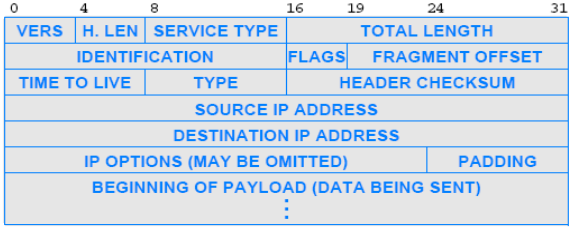
\includegraphics[width=\textwidth]{pic/header_ip.png}
                    \label{Header IP}
                \end{figure}
                \begin{itemize}
                    \item \textbf{VERS} (4 bit)\\
                          Indica la versione del protocollo
                    \item \textbf{H.LEN} (4 bit)\\
                          Specifica la dimensione dell'header ($ tot\_byte\_header/4 $)
                    \item \textbf{SERVICE TYPE} (8 bit)\\
                          Classe di servizio del datagramma
                    \item \textbf{TOTAL LENGTH} (16 bit)\\
                          Numero totale di byte del datagramma
                    \item \textbf{IDENTIFICATION} (16 bit)\\
                          Numero assegnato al datagramma, usato in caso di frammentazione
                    \item \textbf{FLAGS} (3 bit)\\
                          Sono in realtà 3 flag da 1 bit ciascuno. Il primo (\textit{Reserved}) è sempre settato a 0, il secondo (\textit{Don't Fragment}) indica se il datagramma può essere frammentato o meno ed il terzo (\textit{More Fragments}) indica se questo datagramma è l'ultimo di una serie di frammenti
                    \item \textbf{FRAGMENT OFFSET} (13 bit)\\
                          Offset del frammento rispetto al datagramma originale (va moltiplicato per 8 per ottenere il vero offset)
                    \item \textbf{TIME TO LIVE} (8 bit)\\
                          Viene decrementato da ogni router attraverso cui il datagramma passa, se raggiunge 0 questo viene scartato
                    \item \textbf{TYPE} (8 bit)\\
                          Specificano il tipo di dati trasportati dal payload
                    \item \textbf{HEADER CHECKSUM} (16 bit)\\
                          Checksum dell'header
                    \item \textbf{SOURCE IP ADDRESS} (32 bit)\\
                          IP della sorgente
                    \item \textbf{DESTINATION IP ADDRESS} (32 bit)\\
                          IP della destinazione
                    \item \textbf{IP OPTIONS}\\
                          Campi opzionali con informazioni aggiuntive
                    \item \textbf{PADDING}\\
                          Se ho un "IP OPTIONS" valido che non arriva a 32 bit si aggiungono 0 fino a raggiungere quella dimensione
                \end{itemize}

            \subsubsection{Frammentazione IP}
                A seconda della tecnologia HW, i diversi tratti di rete possono avere \textbf{MTU (Maximum Transmission Unit)} diverso. Quando un datagramma ha dimensione maggiore dell'MTU del tratto di rete in cui deve essere inviato il router lo divide in \textit{frammenti} che vengono inviati indipendentemente.\\
                Il router usa quindi il valore dell'MTU per calcolare la dimensione massima di ogni frammento ed il numero effettivo di questi. L'header di ogni frammento è pressochè uguale a quello del datagramma originale (a parte ovvie differenze come \textit{More Fragments} o \textit{Fragment Offset}), ogni frammento porterà nel suo payload una porzione dei dati del datagramma originale.

                \subsubsubsection{Riassemblaggio}
                    Il datagramma verrà riassemblato a destinazione, riducendo così la quantità di dati da memorizzare nel router (\textit{forwarding} non ha bisogno di sapere se un datagramma è frammento o no).\\
                    Ogni frammento viaggia in modo dinamico, se ci fosse un vincolo di passaggio per il riassemblaggio tutti i frammenti dovrebbero passare da quel router, aumentando il traffico.

                \subsubsubsection{Perdita di Frammenti}
                    I datagrammi vengono riassemblati solo quando tutti i frammenti sono arrivati a destinazione. Fino a quel momento questi sono salvati in un buffer, IP specifica un tempo massimo per cui i frammenti vanno conservati (parte all'arrivo del primo frammento).\\
                    Non esistono meccanismi per i quali la destinazione comunichi i frammenti arrivati e se la sorgente ritrasmette il datagramma i suoi frammenti potrebbero seguire percorsi diversi.

            \subsubsection{Indirizzamento a Livello di Rete}
                L'indirizzamento è una componente fondamentale per Internet, infatti vi è uno schema di indirizzamnto comune per tutti gli host.\\
                A questo scopo non possono essere usati i MAC-address del \textit{sotto-livello MAC} in quanto Internet coinvolge vari tipi di tecnologie con (possibilmente) varie tipologie di MAC-address. Per ovviare a questo problema vengono utilizzati gli \textbf{Indirizzi IP}.\\
                A ciascun host viene assegnato un indirizzo univoco a 32 bit, questo dovrà essere specificato quando un host vorrà inviare un datagramma in Internet (\textit{Source IP Address} e \textit{Destination IP Address}, come visto prima nell header).\\
                Gli IP vengono espressi in \textbf{Notazione Decimale Puntata}, gli indirizzi sono divisi in 4 sezioni da \textit{8 bit} ciascuna, delimitate da un punto, con \textit{valore minimo 0} e \textit{valore massimo 255}.\\
                Tra i vari indirizzi IP c'è una gerarchia, infatti gli indirizzi sono divisi in \textit{prefisso} e \textit{suffisso}
                \begin{itemize}
                    \item \textbf{Prefisso}: Identifica la rete fisica a cui un host è connesso
                    \item \textbf{Suffisso}: Identifica un host specifico all'interno di una rete
                \end{itemize} 

                \subsubsubsection{Indirizzamento Classful}
                    Sorge spontanea una domanda, quanti bit devo assegnare al prefisso? E quanti al suffisso?\\
                    Il prefisso deve essere un numero sufficientemente grande per identificare tutte le reti fisiche in Internet, il suffisso deve essere un numero abbastanza grande da esprimere tutti gli host in una rete.\\
                    La soluzione originale al problema prevedeva la divisione dello spazio di indirizzamento in \textit{3 classi primarie}, ciascuna con dimensione di prefisso/suffisso differente. I primi 4 bit di un indirizzo indicavano la classe di appartenenza.\\
                    Metà degli indirizzi esistenti appartenevano alla classe A, con limite a 128 reti, in modo da consentire ai principali ISP di creare la loro rete gigante. Con lo stesso concetto la classe C era pensata per permettere a piccole organizzazioni di creare la loro LAN.\\
                    Venne creata l'\textbf{ICANN (Internet Corporation for Assigned Names and Numbers)} per l'assegnamento degli indirizzi e la soluzione a dispute riguardanti loro. Questa corporation non assegna direttamente i prefissi ma autorizza un insieme di \textit{registrars} a farlo. I registrars assegnano i blocchi agli ISP che li assegnano a loro volta agli utenti.
                    
                \subsubsubsection{Indirizzamneto Classless}
                    Tutti hanno cominciato a chiedere indirizzai di classe A o B, in modo da avere molti indirizzi al fine di espandersi. Ci si ritrovò in una situazione in cui vi era un forte sottoutilizzo degli indirizzi di ogni classe.\\
                    Vennero proposte due soluzioni
                    \begin{itemize}
                        \item Subnet
                        \item Indirizzamento Classless
                    \end{itemize}
                    Si consideri un ISP ed un cliente che chiede un prefisso che può contenere 55 host. Con \textit{classfull}
                    \begin{itemize}
                        \item Indirizzo di classe C
                        \item Sarebbero bastati 6 bit per rappresentarli tutti (190 indirizzi sprecati)
                    \end{itemize}
                    Con \textit{classless} l'ISP può assegnare arbitrariamente la dimensione del prefisso, in questo caso \textit{26 bit di prefisso} e \textit{6 bit di suffisso}.\\
                    Come può un router conoscere la dimensione di un prefisso essendo questo arbitrario di rete in rete? Invece di aggiungere la dimensione del prefisso esplicitamente venne introdotto il concetto di \textbf{Maschera}

                    \paragraph{Maschera}
                        Valore a \textit{32 bit} in cui sono posti a 1 tutti i bit fino a raggiungere la dimensione del prefisso.\\
                    \\
                    Un router tiene in memoria
                    \begin{itemize}
                        \item I prefissi di rete delle destinazioni
                        \item Le corrispondenti maschere
                    \end{itemize}
                    Quando arriva un datagramma con IP generico il router confronta l'indirizzo di destinazione con gli indirizzi che ha in memoria e fa il forward in base alla destinazione.\\
                    Questo confronto non avviene su tutti e 32 i bit, viene infatti considerata la maschera per ogni prefisso con cui fine fatto l'\textit{AND bit-a-bit} nei confronti dell'indirizzo IP. Il risultato viene confrontato con il prefisso in memoria, se sono uguali è stata trovata la destinazione del pacchetto.

                \subsubsubsection{Notazione CIDR}
                    Il \textbf{CIDR (Classless Inter-Domain Routing)} viene espressa nella forma $ ddd.ddd.ddd.ddd/m $, dove
                    \begin{itemize}
                        \item \textit{ddd} è un valore decimale in funzione della notazione decimale puntata
                        \item \textit{m} è in numero di bit del prefisso
                    \end{itemize}
                    Dopo aver ricevuto il \textit{prefisso CIDR da un ISP} si possono assegnare liberamente gli indirizzi host ai propri utenti.

                \subsubsubsection{Indirizzi Speciali}
                    Il protocollo IP definisce una serie di indirizzi riservati detti \textbf{Indirizzi Speciali}
                    \begin{itemize}
                        \item \textbf{Indirizzo di Rete (Suffisso a 0)}: Indica il solo prefisso di una rete, identifica quindi le rete nel complesso. Non deve mai comparire come indirizzo di destinazione di un datagramma.
                        \item \textbf{Directed Broadcast (Suffisso a 1)}: Semplifica il broadcasting, il datagramma con questo indirizzo di destinazione viaggia su Internet fino a raggiungere la rete indicata dal prefisso per poi essere consegnato a tutti gli host della stessa.
                        \item \textbf{Limited Broadcast (Tutti i bit a 1)}: Il datagramma con questo indirizzo come destinazione verrà consegnato a tutti gli host della rete dell'host che ha generato il datagramma. Utilizzato durante lo \textit{startup del sistema}, quando l'host non conosce ancora l'indirizzo di rete.
                        \item \textbf{This Host (Tutti i bit a 0)}: Durante il boot un host non può ancora indicare un indirizzo sorgente corretto in quanto non lo possiede ancora. A tale scopo questo indirizzo indica "This Host", ossia indica lo stesso host che ha generato il datagramma. Non valido come "\textit{Destination IP Address}" di un datagramma.
                        \item \textbf{Loopback (127.0.0.0/8)} Utilizzato per testing, invece che far girare due programmi su host separati il programmatore utilizza un solo host per entrambi ed utilizza quest'indirizzo per farli comunicare. Il suffisso è irrilevante (solitamente si utilizza 127.0.0.1). Di fatto non viene trasmesso alcun datagramma in quanto come viene inviato esso torna a se stesso. 
                    \end{itemize}

                \subsubsubsection{Principi di Indirizzamento}
                    A ciascun router vengono \textit{assegnati 2 o più} IP (uno per ogni rete a cui esso è connesso). Un route infatti ha connessioni verso una o più reti fisiche, il cui indirizzo è specificato in ogni prefisso.\\
                    Quindi un IP non identifica un host specifico ma la connessione tra esso e la rete, quindi un host con più IP avrà un indirizzo per ogni connessione.

        \subsection{ICMP}
            L'\textbf{ICMP (Internet Control Message Protocol)} è un protocollo associato ad IP utilizzato principalmente per inviare messaggi di errore alla sorgente in caso di problemi. Questi due protocolli dipendono uno dall'altro
            \begin{itemize}
                \item IP dipende da ICMP per l'invio di messaggi d'errore
                \item ICMP dipende da IP per trasportare i messaggi di errore
            \end{itemize}
            Ecco alcuni messaggi
            \begin{figure}[H]
                \centering
                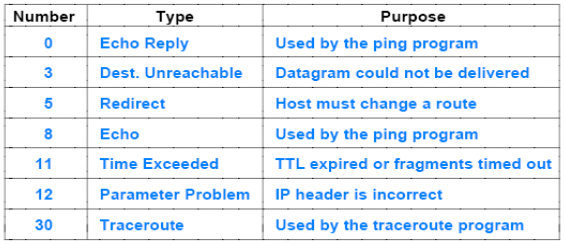
\includegraphics[width=\textwidth]{pic/messaggi_icmp.png}
                \label{Messaggi ICMP}
            \end{figure}
            Abbiamo due tipologie di messaggi
            \begin{itemize}
                \item Messaggi per \textit{segnalazione errori}
                \item Messaggi per \textit{ottenere informazioni}
            \end{itemize}
            Come detto prima ICMP usa IP per trasportare i propri messaggi, mettendo il messaggio ICMP nel payload del datagramma IP che verrà inviato come ogni altro datagramma. Se un messaggio ICMP genera un errore non verrà inviato alcun errore per evitare "l'effetto valanga".
            \begin{figure}[H]
                \centering
                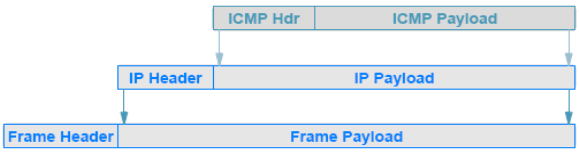
\includegraphics[width=\textwidth]{pic/icmp_ip.png}
                \label{Messaggio ICMP dentro datagramma IP}
            \end{figure}

        \subsection{DHCP}
            Quando un host o un router vengono accesi il Sistema Operativo ed il SW che gestisce il protocollo di rete vengono inizializzati.\\
            Chi gestisce un router deve specificare dei valori iniziali, quali
            \begin{itemize}
                \item L'indirizzo per ciascuna connessione di rete (interfaccia)
                \item Quale SW di protocollo utilizzare
                \item I valori iniziali delle tabelle di forwarding
            \end{itemize}
            Questa configurazione viene salvata e caricata dal router durante lo startup.\\
            La configurazione degli host segue un processo noto come \textbf{bootstrapping}. È stato ideato un protocollo che permette ad un host di ottenere una serie di parametri con una singola richiesta, chiamato \textbf{BOOTP (Bootstrap Protocol)}.\\
            Attualmente è il DHCP che viene usato per fornire la maggioranza delle informazioni di configurazione.\\
            \\
            Il \textbf{DHCP (Dynamic Host Configuration Protocol)} viene utilizzato per permettere ad un host di una rete di ricevere automaticamente, ad ogni richiesta d'accesso, la configurazione IP necessaria per stabilire una connessione e inter-operare con tutte le altre sotto-reti, purchè anch'esse integrate nello stesso modo con IP.\\
            Sono stati creati vari meccanismi per permettere ad un host di ottenere i diversi parametri
            \begin{itemize}
                \item \textbf{RARP (Reverse Address Resolution Protocol)} permette di ottenere un indirizzo IP da un server
                \item \textbf{ICMP} ha i messaggi "\textit{Address Mask Request}" e "\textit{Router Discovery}" utilizzati, rispettivamente, per ottenere la maschera della rete e l'indirizzo del router 
            \end{itemize}
            DHCP utilizza un approccio "\textit{Plug-and-Play Networking}", infatti permette di ottenere molte di queste informazioni e quelle sopracitate automaticamente.\\
            \\
            Quando un host si accende
            \begin{itemize}
                \item Invia in \textit{broadcast} una \textbf{DHCP-Request}
                \item Il server risponde con una \textbf{DHCP-Response}
                      \begin{itemize}
                          \item DHCP chiama "\textit{offerta}" il messaggio inviato dal server
                          \item Si dice, infatti, che il server stia \textit{offrendo} un indirizzo al client
                      \end{itemize}
            \end{itemize}
            Si può configurare DHCP per fornire due tipi di indirizzi
            \begin{itemize}
                \item Indirizzi assegnati permanentemente (come \textbf{BOOTP})
                \item Indirizzi dinamici scelti da un insieme allocato appositamente
            \end{itemize}
            Come regola generale, gli indirizzi permanenti si assegnano a server mentre quelli dinamici ad host generici (assegnati solo per un tempo predeterminato, "\textbf{lease}").\\
            Quando il periodo di lease scade il server considera come libero quell'indirizzo, l'host può quindi rinunciarvi o rinegoziare con il server un'estensione del periodo di lease (solitamente approvate). Questo non vuol dire che DHCP non possa essere configurato per \textit{negare} sempre le suddette richieste.\\
            \\
            In caso di perdita o duplicazione di pacchetti DHCP non vi è alcun errore, se un host non riceve \textit{Response} re-invia la \textit{request}, se invece riceve duplicati li ignora.\\
            Quando un host trova un server DHCP lo memorizza per utilizzi futuri. Non è possibile che due \textit{DHCP-Request} arrivino in contemporanea.
            
            \subsubsection{Formato dei messaggi}
                \begin{figure}[H]
                    \centering
                    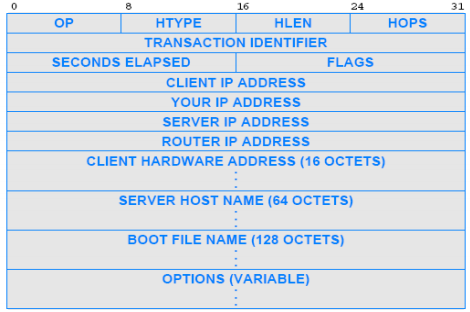
\includegraphics[width=\textwidth]{pic/messaggio_dhcp.png}
                    \label{Messaggio DHCP}
                \end{figure}
                Versione leggermente modificata dei messaggi BOOTP
                \begin{itemize}
                    \item \textbf{OP} (8 bit)\\ 
                          Indica se il messaggio è \textit{Request} o \textit{Response}
                    \item \textbf{HTYPE} (8 bit)\\
                          Indica il tipo HW della rete
                    \item \textbf{HLEN} (8 bit)\\
                          Indica la lunghezza dell'indirizzo HW
                    \item \textbf{FLAGS} (16 bit)\\
                          Indica se l'host può ricevere \textit{messaggi broadcast} o \textit{risposte dirette}
                    \item \textbf{HOPS} (8 bit)\\
                          Indica a quanti server rigirare la richiesta
                    \item \textbf{TRANSACTION IDENTIFIER} (32 bit)\\
                          Indica il valore, usato da un host, per capire se una risposta si riferisce ad una sua richiesta
                    \item \textbf{SECONDS ELAPSED} (16 bit)\\
                          Indica quanti secondi sono passati dall'avvio dell'host
                \end{itemize}
                I campi finali si usano per trasportare le informazioni di risposta verso la sorgente
                \begin{itemize}
                    \item \textbf{YOUR IP ADDRESS} (32 bit)\\
                          Se un host non conosce il proprio IP, il server usa questo campo per indicarglielo
                    \item \textbf{SERVER IP ADDRESS} (32 bit)\\
                          Fornisce l'IP del server DHCP contattato
                    \item \textbf{SERVER HOST NAME} (512 bit)\\
                          Fornisce l'Host Name del server DHCP contattato
                    \item \textbf{ROUTER IP ADDRESS} (32 bit)\\
                          Indirizzo IP del router di default
                \end{itemize}

        \subsection{Carenza di Indirizzi IP}
            Il protocollo IP usa 32 bit per l'indirizzamento, all'epoca della sua introduzione sembravano più che sufficienti, ora invece la crescita esponenziale di Internet ha posto il problema della loro carenza.

            \subsubsection{NAT}
                Lo \textbf{IETF (Internet Engeneering Task Force)} ha definito alcuni range di indirizzi da utilizzare solo in ambito privato, ogni volta che un pacchetto con \textit{IP privato} viene consegnato ad un \textit{router pubblico} viene segnalato un errore.\\
                Gli \textbf{Indirizzi IP privati} vengono utilizzati in reti con un solo (o pochi) punto d'accesso ad Internet. Viene per questo introdotto il \textbf{NAT (Network Address Translation)} con il fine di risolvere i problemi di instradamento tra \textit{reti ad indirizzamento pubblico} e \textit{reti ad indirizzamento privato}.

                \paragraph{Datagrammi Uscenti}
                    NAT sostituisce \textit{l'indirizzo sorgente} dei datagrammi uscenti con il proprio \textit{IP pubblico}

                \paragraph{Datagrammi Entranti}
                    NAT sostituisce \textit{l'indirizzo di destinazione} dei datagrammi entranti con l'\textit{IP privato} dell'host corretto

                \subsubsubsection{NAT Table}
                    Il router abilitato NAT (router di confine) mantiene al suo interno una tabella in cui tiene traccia dei mapping tra \textit{IP privato} delle sorgenti ed \textit{IP pubblico} delle destinazioni. Questa tabella può essere aggiornata in due modi
                    \begin{itemize}
                        \item \textbf{Manualmente}: Il gestore della rete configura staticamente i record della NAT Table
                        \item \textbf{Dinamicamente}: Ogni volta che un datagramma uscente passa per il router NAT viene creato un record della tabella. Questi vengono cancellati con un meccanismo di \textit{timeout}
                    \end{itemize} 
                    Il NAT basato unicamente su indirizzo non permette a diversi host privati di connettersi contemporaneamente allo stesso host pubblico
                    
            \subsubsection{NAPT}
                Il \textbf{NAPT (Network Addres and Port Translation)} è un evoluzione nel NAT che permette al router di agire da \textit{gateway di livello 4}, traducendo sia IP che numero di Porta. Il funzionamento è analogo a quello di NAT.

            \subsubsection{IPv6}
                Mantiene molte caratteristiche di IPv4 (attuale implementazione), tra cui
                \begin{itemize}
                    \item Connectionless
                    \item Hop massimi per ogni datagramma
                \end{itemize}
                Molte funzionalità, però, sono cambiate.\\
                Gli indirizzi IPv6 sono formati da \textbf{128 bit}, hanno un formato dell'header diverso e introduce il concetto di "\textbf{Extension Header}", un datagramma IPv6 quindi è formato da un \textit{header}, \textit{extension header} (facoltativo) ed i dati inviati.\\
                Questa versione del protocollo introduce il supporto del traffico Real-Time, ossia viene introdotto un meccanismo che permette di creare un cammino tra sorgente e destinazione, potendo associare i datagrammi a tale cammino (per applicazioni che richiedono maggiore qualità del servizio).

                \subsubsubsection{Formato dei Datagrammi}
                    \begin{figure}[H]
                        \centering
                        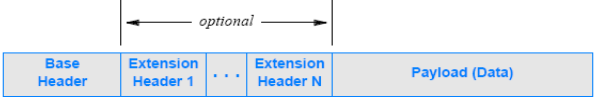
\includegraphics[width=\textwidth]{pic/ipv6_datagram.png}
                        \label{Datagramma IPv6}
                    \end{figure}

                    \paragraph{Header di Base}
                        \begin{figure}[H]
                            \centering
                            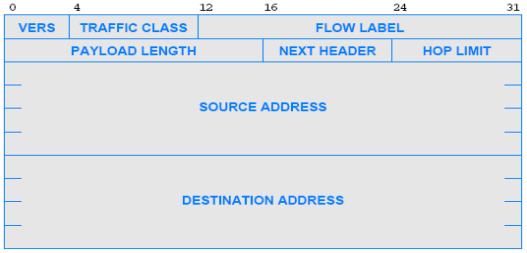
\includegraphics[width=\textwidth]{pic/base_header_ipv6.png}
                            \label{Header di base IPv6}
                        \end{figure}
                        \begin{itemize}
                            \item \textbf{VERS} (4 bit)\\
                                  Versione 6
                            \item \textbf{TRAFFIC CLASS} (8 bit)\\
                                  Classe di traffico in base al tipo di traffico, specifica i requisiti che la rete fovrebbe soddisfare
                            \item \textbf{PAYLOAD LENGHT} (16 bit)\\
                                  Dimensione del payload
                            \item \textbf{HOP LIMIT} (8 bit)\\
                                  Corrisponde al TIME-TO-LIVE di IPv4
                            \item \textbf{FLOW LABEL} (20 bit)\\
                                  Associa un datagramma ad un cammino specifico
                            \item \textbf{NEXT HEADER} (8 bit)\\
                                  Specifica il tipo di informazione che segue l'header corrente, se ho \textit{Extension Header} ne indica il tipo, se non ne ho indica il tipo di dati nel payload
                            \item \textbf{SOURCE/DESTINATION ADDRESS} (128+128 bit)\\
                                  Indirizzo sorgente e destinazioen del datagramma
                        \end{itemize}
\newpage
                    
                    \paragraph{Extension Header} 
                        \begin{figure}[H]
                            \centering
                            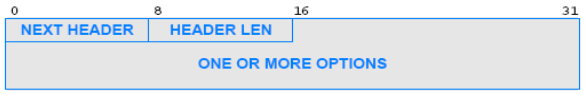
\includegraphics[width=\textwidth]{pic/extension_header_ipv6.png}
                            \label{Extension Header IPv6}
                        \end{figure}
                        \begin{itemize}
                            \item \textbf{NEXT HEADER} (8 bit)\\
                                  Esiste un valore unico per ogni header possibile, indica il valore del prossimo header
                            \item \textbf{HEADER LEN} (8 bit)\\
                                  Dimensione dell'Extension Header, può variare di header in header
                        \end{itemize}
                    Perchè inserire header multipli? In quanto si risparmia spazio (vengono utilizzate sempre solo un sottinsieme delle funzionalità), si possono inoltre aggiungere funzionalità senza che ogni header abbia informazioni al riguardo pur non utilizzandole.

                \subsubsubsection{Frammentazione}
                    Simile alla frammentazione IPv4.\\
                    Come in IPv4
                    \begin{itemize}
                        \item Il prefisso del datagramma originale è copiato in ogni frammento
                        \item La dimensione varia in base alla MTU della rete
                    \end{itemize}
                    Diversamente da IPv4
                    \begin{itemize}
                        \item Non esistono campi dell'header riguardanti la frammentazione, queste vanno infatti aggiunte in un extension header di tipo "\textit{frammentazione}"
                    \end{itemize}

                \subsubsubsection{Indirizzamento}
                    Come con CIDR, la divisione tra \textit{prefisso} e \textit{suffisso} è arbitraria. IPv6 introduce il concetto di \textbf{Gerarchia Multilivello}
                    \begin{itemize}
                        \item Il livello più alto è per gli ISP
                        \item Livello successivo per organizzazioni
                        \item Livello successivo per siti specifici
                        \item E così via fino agli host locali
                    \end{itemize}

                    \paragraph{Indirizzi Speciali}
                        \begin{itemize}
                            \item \textbf{Unicast}: Corrisponde ad un singolo host. Datagramma instradato verso tale indirizzo segue il cammino minimo
                            \item \textbf{Multicast}: Corrisponde ad un insieme di host che possono variare in qualsiasi momento. Viene consegnata una copia del datagramma ad ogni membro dell'insieme
                            \item \textbf{Anycast}: Corrisponde ad un insieme di host che condividono lo stesso prefisso. Il datagramma viene consegnato ad uno qualsiasi degli host dell'insieme
                        \end{itemize}

                    \paragraph{Notazione Esadecimale}
                        Nell'indirizzo IPv6 ciascun gruppo di \textit{16 bit} viene separato dal carattere ":". Le sequenze di zeri si possono comprimere
                        \begin{center}
                            \underline{\textbf{Esempio}}: FF0C:0:0:0:0:0:0:B1 $ \rightarrow $ FF0C : : B1
                        \end{center}
                        Questo facilita la transizione, infatti per trasporre gli indirizzi IPv4 esistenti basta porre a 0 i primi \textit{96 bit}

\newpage                        
    \section{Livello Data-Link}
        L'obiettivo del livello \textbf{Data-Link} è quello di fornire al livello di Rete una connessione il più possibile affidabile tra due macchine adiacenti.\\
        Per \textit{Macchine Adiacenti} si intende connesse da un canale di comunicazione, sia esso fisico o wireless. Condizione necessaria è però che questo canale sia quello che possiamo definire "\textit{tubo digitale}", ossia che l'ordine dei bit venga rispettato e quindi essi arrivino a destinazione come sono stati inviati.

        \subsection{Tipologia di servizi offerti al livello superiore}
            \begin{itemize}
                \item \textbf{Servizio Connectionless senza Acknowledge} \\
                      Nessuna connessione viene attivata e non si attende alcun \textit{feedback} dalla destinazione. Se una trama viene persa non ci sono tentativi per recuperala, questo compito viene lasciato ai livelli superiori.
                \item \textbf{Servizio Connectionless con Acknowledge} \\
                      Nessuna connessione viene attivata ed ogni trama inviata viene riscontrata in maniera individuale.
                \item \textbf{Servizio Connection-Oriented con Acknowledge} \\
                      Viene attivata una connessione e, al termine del trasferimento, essa viene abbattuta. Anche in questo caso ogni trama viene riscontrata in maniera individuale.
            \end{itemize}

        \subsection{Funzionalità del Livello Data-Link}
            \begin{itemize}
                \item \textbf{Framing} \\
                      Delimitazione delle trame
                \item \textbf{Rilevazione/Gestione Errori} \\
                      Viene effettuato un controllo sul contenuto della trama, in caso vi fossero errori gestisce il recupero della stessa
                \item \textbf{Controllo di Flusso} \\
                      Gestisce la velocità di trasmissione
            \end{itemize}

        \subsubsection{Framing}
            Bisogna tenere conto del fatto che la lunghezza dei pacchetti ricevuti del \textit{Livello di Rete} e delle corrispondenti trame di \textit{Livello Data-Link} può variare. Inoltre, dato che il \textit{Livello Fisico} tratta solo bit non è possibile distinguere dove termina una trama e dove comincia la successiva. \\
            Il \textbf{framing} si occupa proprio di rendere distinguibile una trama dall'altra attraverso l'utilizzo di opportuni codici all'inizio o alla fine di ogni \textit{frame}.

            \subsubsubsection{Modalità di Framing}
                Ho più modi per implementare il \textit{framing}:
                \begin{itemize}
                    \item Posso inserire intervalli temporali tra trame consecutive
                          \begin{itemize}
                              \item \underline{Problema}: Per natura delle reti non viene data alcuna garanzia sul rispetto delle caratteristiche temporali, quindi l'intervallo inter-trama potrebbe essere esteso o ridotto generando problemi di ricezione. 
                          \end{itemize}
                    \item Posso marcare l'inizio e la fine di ogni trama
                          \begin{itemize}
                              \item Character Count
                              \item Bit Stuffing
                          \end{itemize}
                \end{itemize}
                
                \paragraph{Character Count}Un campo nell'header del frame indica il numero di caratteri nel frame stesso

                \paragraph{Bit Stuffing}Ogni trama ha un numero arbitrario di bit. In questa modalità di \textit{framing} ogni trama inizia con un particolare pattern (\textit{01111110}) chiamato \textit{Byte di Flag}.\\
                Sorge spontaneo un dubbio, come mi comporto se la trama contiene già la sequenza di bit 01111110? In questo caso, ossia se vengono trovati cinque $ 1 $ consecutivi, viene aggiunto uno 0. Questo 0 aggiuntivo verrà poi tolto al momento della ricezione.

        \subsubsection{Rilevazione degli errori}
            Posso avere diverse tipologie di errori, essi possono essere:
            \begin{itemize}
                \item Errori sul singolo bit
                \item Replicazione di bit
                \item Perdita di bit
            \end{itemize}
            Al fine di rilevare questi errori è stato inserito un campo dell'header detto \textbf{checksum}. Esso è il risultato di un calcolo fatto utilizzando i bit della trama. La destinazione, una volta ricevuta la trama ripete il calcolo, se il valore ottenuto coincide con quello nel campo checksum allora la trama è corretta. 

        \subsubsection{Gestione del Flusso}
            Può capitare che la sorgente invii trame ad una velocità superiore a quella con cui la destinazione può riceverle. La conseguenza diretta di questo fatto è una congestione del nodo destinazione. Il \textit{Controllo di Flusso} è implementato in modo da controllare la velocità di trasmissione della sorgente in base al feedback inviatigli dalla destinazione. Questo feedback può dare istruzione di:
            \begin{itemize}
                \item Bloccare la trasmissione fino al comando successivo
                \item Limitare la quantità di informazione inviata in base a quanta ne è ancora in grado di gestire la destinazione
            \end{itemize}
            Nelle reti \textbf{TCP/IP} il controllo di flusso e di recupero errori è affidato ai livelli superiori
    
\newpage            
    \section{Il sotto-livello MAC}
        Il mezzo fisico, con cui il \textit{Livello Data-Link} si interfaccia, è collegato anch'esso tramite un mezzo fisico. Questo può essere:
        \begin{itemize}
            \item \textit{Dedicato} (reti punto-punto)
            \item \textit{Condiviso} (reti broadcast)
        \end{itemize}
        Se il mezzo fisico è condiviso nascono delle problematiche legate all'accesso, bisognerà infatti selezionare l'host che ha diritto di trasmettere sul mezzo condiviso, creando una situazione di contesa per la risorsa trasmissiva. \\
        Viene per questo introdotto un sotto-livello al Data-Link che gestisce queste problematiche: il \textbf{sotto-livello MAC (Medium Access Control)}. \\
        \\
        Per mezzo condiviso si intende che un singolo canale trasmissivo può essere utilizzato da più sorgenti. Naturale quindi comprendere il fatto che se ogni partecipante alla comunicazione inviasse informazioni contemporaneamente nessuna di queste sarebbe distinguibile dalle altre. \\
        Necessitiamo quindi una serie di regole per poter utilizzare il mezzo, dette \textit{Tecniche di Allocazione del Canale}.

        \subsection{Tecniche di Allocazione}
            Esistono due categorie di tecniche:
            \begin{itemize}
                \item \textbf{Allocazione Statica} \\
                      Il mezzo trasmissivo viene "\textit{partizionato}" ed ogni porzione viene data alle diverse sorgenti. Questo può avvenire in base:
                      \begin{itemize}
                          \item \underline{al tempo}: Ogni sorgente ha a disposizione il mezzo per un dato periodo di tempo
                          \item \underline{alla frequenza}: Ogni sorgente ha a disposizione una determinata frequenza
                      \end{itemize}
                \item \textbf{Allocazione Dinamica} \\
                      Il canale viene allocato di volta in volta a chi ne fa richiesta e può essere utilizzato da un'altra sorgente solo dopo che la prima finisce di utilizzarlo e lo libera.                     
            \end{itemize}

            \subsubsection{Allocazione Statica}
                Vale la pena usare questa tecnica di allocazione nel caso un cui ci si trovi con pochi utenti e questi abbiano grossi carichi di informazioni da inviare che però sono costanti nel tempo. Se le risorse vengono date ad utenti che non le utilizzano, quindi non inviano niente, queste sono effettivamente \textit{perse}.
            
            \subsubsection{Allocazione Dinamica}
                Il canale trasmissivo può essere assegnato:
                \begin{itemize}
                    \item \textbf{A turno}: Viene distribuito il "\textit{permesso}" di trasmettere, la durata viene decisa dalla sorgente
                    \item \textbf{A contesa}: Ogni sorgente prova a trasmettere indipendentemente dalle altre
                \end{itemize}
                Nel promo caso si sottintende la presenza di un \textit{Overhead di Gestione}, ossia di un meccanismo per l'assegnazione del permesso per trasmettere. Nel secondo caso, invece, non c'è nessun meccanismo di assegnazione al fine di mantenere sorgente e destinazione i più semplici possibile. La \textit{Trasmissione a Contesa} è generalmente la più utilizzata.

        \subsection{Protocolli di Accesso Multiplo}
            Principali algoritmi usati dai protocolli:
                \begin{itemize}
                    \item \textbf{ALOHA}
                          \begin{itemize}
                              \item Pure ALOHA
                              \item Slotted ALOHA
                          \end{itemize}
                    \item \textbf{Carrier Sense Multiple Access Protocols}
                          \begin{itemize}
                              \item CSMA
                              \item CSMA-CD (Collision Detection)
                          \end{itemize}
                \end{itemize}

            \subsubsection{Pure ALOHA}
                Definito nel 1970 dall'Università delle Hawaii \\
                \underline{Algoritmo}:
                \begin{itemize}
                    \item Una sorgente può trasmettere una trama ogniqualvolta vi sono dati da inviare (\textit{continuous time})
                    \item La sorgente rileva, ascoltando il canale, l'eventuale collisione
                    \item Se avviene una collisione, la sorgente aspetta un tempo casuale per poi ritrasmettere la trama
                \end{itemize}
                Il \textbf{Periodo di Vulnerabilità} per il Pure ALOHA, che è l'intervallo di tempo in cui possono avvenire delle collisioni, e 2T (con T = \textit{Tempo di Trama}, ossia il tempo necessario per trasmettere una trama).

            \subsubsection{Slotted ALOHA}
                Proposto nel 1972 da Roberts per duplicare la capacità di Pure ALOHA.\\
                L'algoritmo si basa sulla divisione del tempo in intervalli discreti. La differenza sta proprio in questo, infatti esso si comporta come il Pure ALOHA ma una trama può essere inviata solo ad intervalli di tempo definiti, è dunque necessario che vi sia sincronizzazione tra due stazioni.\\
                Di conseguenza il \textbf{Periodio di Vulnerabilità} è T (\textit{Tempo di Trama}).

            \subsubsection{Carrier Sense Multiple Access (CSMA)}
                Ci troviamo ora nell'ambito delle LAN, dove le stazioni possono monitorare lo stato del canale di trasmissione. Le stazioni ascoltano il canale \textit{prima} di iniziare a trasmettere per verificare se sta avvenendo una trasmissione.\\
                \underline{Algoritmo}:
                \begin{itemize}
                    \item Se il canale è libero si trasmette
                    \item Se esso è occupato, sono possibili diverse varianti
                          \begin{itemize}
                              \item \textbf{Non-persistent}: Rimanda la trasmissione ad un nuovo istante, scelto in maiera casuale
                              \item \textbf{Persistent}: Nel momento in cui il canale torna libero la stazione inizia a trasmettere
                          \end{itemize}
                    \item Se avviene una collisione si comporta come ALOHA
                \end{itemize}

            Vi sono alcune varanti del CSMA, che verranno illustrate nelle sezioni a seguire
            
            \subsubsection{CSMA P-Persistent}
                Il tempo viene suddiviso in intervalli, la misura degli intervalli coincide con il periodo di vulnerabilità, ossia 2$\tau$. \\
                \underline{Algoritmo}:
                \begin{enumerate}
                    \item Ascolta il canale
                        \begin{itemize}
                            \item Se il canale è libero:
                                  \begin{itemize}
                                    \item Si trasmette con probabilità P
                                    \item Se si è deciso di trasmettere, si passa al punto 2
                                    \item Se si è deciso di non trasmettere si attende un intervallo di tempo e si torna al punto 1
                                  \end{itemize}
                            \item Se è occupato si attende un intervallo di tempo e si torna al punto 1 
                        \end{itemize} 
                    \item Se c'è collisione
                        \begin{itemize}
                            \item Si attende un tempo casuale e si torna al punto 1
                        \end{itemize}
                \end{enumerate}
                Il periodo di vulnerabilità è legato al \textit{Ritado di Propagazione} ($\tau$). Infatti, se una stazione ha iniziato a trasmettere ma il suo segnale non è ancora arrivato a tutte le stazioni, qualcun altro potrebbe iniziare la trasmissione. In genere il \textit{Ritardo di Propagazione} è molto inferiore al \textit{Tempo di Trama} (T)

            \subsubsection{CSMA con Collision Detection (CSMA-CD)}
                Rispetto al P-Persistent esso migliora in quanto riesce a rilevare le collisioni e bloccare la trasmissione immediatamente. In questo modo non vi è spreco di tempo. Dopo aver interrotto la trasmissione invia una sequenza, detta \textit{Sequenza di Jamming}, per segnalare alle altre stazioni l'avvenuta collisione.
                
        \subsection{LAN Estese}
            La rappresentazione tipica di una LAN è una serie di stazioni (PC) connesse ad un segmento di cavo (Bus). Poichè questo segmento di cavo non può essere troppo lungo, nel tempo, è nato il problema di estendere le LAN. Per fare questo si sfruttano tre tipi di apparati:
            \begin{itemize}
                \item Repeater o Hub
                \item Bridge
                \item Switch
            \end{itemize} 

            \subsubsection{Dominio di Collisione}
                Parti di rete per cui, se due stazioni trasmettono contemporaneamente, il segnale ricevuto da queste risulta danneggiato.
            
            \subsubsection{Dominio di Broadcast (Segmento Data-Link)}
                Parte di rete raggiunta da una trama con indirizzo di broadcast, se due stazioni appartengono alla stessa rete di Livello Data-Link, due stazioni hanno lo stesso dominio di broadcast.

            \subsubsection{Repeater o Hub}
                Apparato che interviene solo a Livello Fisico. Esso replica le trame in arrivo da un segmento ad un altro, amplificando il segnale. \\
                Se un Repeater collega \textit{due o più segmenti} si parla di \textbf{Hub}, che copia la trama ricevuta e la ripete su tutte le porte.

            \subsubsection{Bridge}
                Collega due segmenti di rete. A differenza delle Repeater, il Bridge è un apparato intelligente. \\
                Seleziona, basandosi su una tabella da lui stesso mantenuta in cui si tiene traccia del segmento di rete di appartenenza per ciascuna rete, se ripetere una trama generata da un segmento di rete su un altro segmento di rete. Grazie al Bridge si può spezzare il dominio di collisione.

            \subsubsection{Switch}
                Può essere visto come un Bridge multiporta. Spesso ad ogni porta è associata una ed una sola stazione. Riesce quindi a realizzare un accesso dedicato per ogni nodo, eliminando le collisioni potendo quindi sopportare conversazioni contemporanee multiple.

        \subsection{Incapsulamento IP}
            Il Livello Data-Link svolge una serie di funzionalità che permettono il trasferimento \textit{hop-by-hop}. Ognuno di questi hop può avere un protocollo di Livello 2 diverso da quello dell'hop successivo.\\
            Esistono diverse modalità di incapsulamento IP:
            \begin{itemize}
                \item \underline{Soluzioni per l'accesso}
                      \begin{itemize}
                          \item Ethernet e 802.3
                          \item PPP
                                \begin{itemize}
                                    \item PPP con Modem
                                    \item PPP con ADSL
                                \end{itemize}
                      \end{itemize}
                \item \underline{Soluzioni per il backbone}
                      \begin{itemize}
                          \item Frame Relay
                          \item ATM
                          \item Soluzioni su SDH
                      \end{itemize}
            \end{itemize}

            \subsubsection{Ethernet e 802.3}
                Si interfaccia direttamente con il Livello Fisico sopportando un carico del 30\% (3 Mb/s) con picchi del 60\% (6 Mb/s). A livello statistico, sotto carico medio, il 2/3\% collide una volta e solo qualche pacchetto su 10000 ha collisioni multiple.\\
                Gli standard Ethernet e 802.3 implementano un livello MAC di tipo \textit{CSMA/CD 1-persistent}. In caso di collisione, l'istante in cui ritrasmettere viene calcolato tramite un algoritmo di \textit{Binary Exponential Backoff}
                \begin{itemize}
                    \item Dopo le collisioni, l'host attende un intervallo di tempo casuale prima di ri-trasmettere, estraendo un numero casuale nell'intervallo [0, 1, ..., $ 2^i - 1 $]
                    \item \underline{Vincoli}
                          \begin{itemize}
                              \item Dopo 10 collisioni, tempo d'attesa limitato tra [0, 1, ..., 1023]
                              \item Dopo 16 collisioni, viene riportata una \textbf{failure} al Sistema Operativo
                          \end{itemize}
                \end{itemize}

                Il formato della trama è il seguente
                \begin{figure}[H]
                    \centering
                    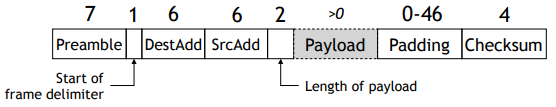
\includegraphics[width=\textwidth]{pic/trama_802.png}
                    \label{Trama 802.3}
                \end{figure}
                \begin{itemize}
                    \item \textbf{Preamble} (7 Byte) \\
                          Si usa per sincronizzare il ricevitore
                    \item \textbf{Start of Frame} (1 Byte) \\
                          Flag di inizio trama
                    \item \textbf{Destination Address} (6 Byte) \\
                          Indirizzo di destinazione della trama
                    \item \textbf{Source Address} (6 Byte) \\
                          Indirizzo sorgente della trama
                    \item \textbf{Length} (2 Byte) \\
                          Lunghezza in Byte della trama, tra 0 e 1500 (se $ >1500 $ indica \textit{Protocol Type})
                    \item \textbf{Payload} \\
                          Informazione Trasmessa
                    \item \textbf{Checksum} \\
                          Codice per rilevamento errori
                \end{itemize}

            \subsubsection{PPP}
                PPP viene utilizzato sia nell'accesso che nel backbone. Esso è un protocollo \textit{Charachter Oriented} e utilizza il \textit{Bit Stuffing} per il framing. \\
                Il formato della trama è il seguente
                \begin{figure}[H]
                    \centering
                    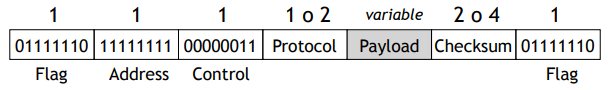
\includegraphics[width=\textwidth]{pic/trama_ppp.png}
                    \label{Trama PPP}
                \end{figure}
                \begin{itemize}
                    \item \textbf{Flag} (1 Byte) \\
                          Identifica inizio e fine della trama (\textit{Bit Stuffing})
                    \item \textbf{Address} (1 Byte) \\
                          Utilizzato in configurazione "\textit{Tutti gli Host}"
                    \item \textbf{Control} (1 Byte)
                          \begin{itemize}
                              \item Valore predefinito 00000011 con il significato di \textit{unnumbered}
                              \item Di default non fornisce un sevizio affidabile in quanto le richieste di ritrasmissione e rimozione duplicati sono lasciate ai livelli superiori 
                          \end{itemize}
                    \item \textbf{Protocol} (1 o 2 Byte) \\
                          Identifica il tipo di livello della trama 
                    \item \textbf{Payload} \\
                          Informazione trasmessa
                    \item \textbf{Checksum} (2 o 4 Byte) \\
                          Identificazione errori
                \end{itemize}
                L'accesso può avvenire con Modem o xDSL
                \begin{itemize}
                    \item \underline{Modem}: Utilizza la banda telefonica, ha un limite superiore di \textit{56k} 
                    \item \underline{xDSL (Digital Subscriber Line)}: Famiglie di tecnologie che permettono di utilizzare la banda disponibile del doppino telefonico. Possono esserci sistemi \textit{Simmetrici e Asimmetrici}.\\
                          Per esempio, \textit{ADSL} e un Sistema Simmetrico su Singola Coppia, è \textit{Rate Adaptive}, va dai 640 agli 8200 Kb/s in upstream e fino a 512 Kb/s in upstream.  
                \end{itemize}

        \subsection{Address Resolution Protocol}
            Ogni scheda di rete ha un indirizzo univoco associato chiamato indirizzo MAC. Questo viene creato e assegnato al momento della produzione della scheda di rete. Necessitiamo dell'indirizzo MAC per la \textit{consegna diretta/indiretta}.

            \subsubsection{Consegna Diretta}
                Sorgente e destinazione appartengono alla stessa rete e quindi il pacchetto può essere inviato direttamente alla destinazione

            \subsubsection{Consegna Indiretta}
                Sorgente e destinazione non appartengono alla stessa rete, la sorgente manda le trame al router che si farà carico della consegna. Per consegnare le trame al router si utilizza l'indirizzo MAC. \\
                Il router riceve una trama che contiene come indirizzo MAC di destinazione quello del router. Il Livello Data-Link estrae il payload e passa al Livello di Rete. \\
                Il router controlla l'IP di destinazione, se non è il suo indirizzo IP allora va consegnato al router successivo. Per fare questo controlla le tabelle di routing per trovare il \textit{next-hop}. Incapsula quindi il pacchetto in una nuova trama con indirizzo MAC di destinazione quello del prossimo router.
                
            \subsubsection{Risoluzione degli indirizzi}
                Dato un indirizzo IP come posso risalire al suo MAC? Utilizzo \textbf{ARP (Address Resolution Protocol)}. \\
                Un host può risolvere l'indirizzo di un altro host solo se entrambi sono collegati alla stessa rete fisica. \\
                Supponiamo che un host A voglia risolvere l'indirizzo IP di un host B:
                \begin{itemize}
                    \item A invia una richiesta in broadcast che chiedendo l'indirizzo MAC dell'host con indirizzo IP:B
                    \item Il broadcast (Limitato) viaggia solo sulla rete locale, quindi raggiungerà tutti gli host della rete
                    \item Quando l'host B riceverà la richiesta risponderà direttamente ad A (quindi non in broadcast) dandogli il proprio indirizzo MAC
                \end{itemize}

            \subsubsection{ARP Caching e Processing dei Messaggi}
                Inviare una richiesta ARP per ogni datagramma sarebbe inefficiente in quanto avremmo tre trame che viaggiano per ogni datagramma: una richiesta ARP, una risposta ARP e la trama con i dati.\\
                Per ridurre il traffico nella rete, ARP estrae e salva le informazioni delle risposte ARP, queste verranno mantenute in memoria tramite una tabella. Questa viene gestita come una cache, ogni associazione IP $ \rightarrow $ MAC viene aggiornata quando si riceve una risposta, se la tabella è piena si rimuove l'entry più vecchia. Se invece una entry non viene aggiornata per molto tempo essa viene rimossa. \\
                Prima di inviare una richiesta ARP, ogni host controlla che non ci sia già una entry per l'associazione che sta cercando nella tabella ARP, se l'informazione è presente l'associazione viene utilizzata senza inviare alcuna richiesta, altrimenti viene inviata la richiesta ed al momento della risposta la cache viene aggiornata e si utilizza l'informazione appena ottenuta per inviare la trama.
                
            \subsubsection{Formato dei messaggi}
                ARP non risolve solo IP e MAC, lo standard è generale e specifica messaggi diversi in base ai protocolli coinvolti.
                \begin{figure}[H]
                    \centering
                    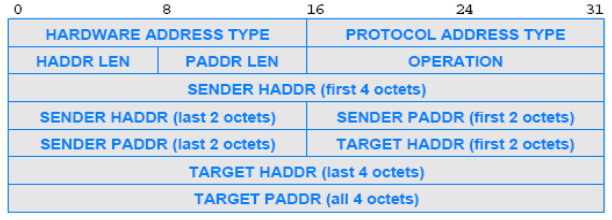
\includegraphics[width=\textwidth]{pic/arp.png}
                    \label{Messaggio ARP}
                \end{figure}
                \begin{itemize}
                    \item \textbf{HARDWARE ADDRESS TYPE} (16 bit) \\
                          Tipo di indirizzo HW utilizzato ($ =1 $ se Ethernet)
                    \item \textbf{PROTOCOL ADDRESS TYPE} (16 bit) \\
                          Tipo di indirizzo del protocollo utilizzato (0x0800 se IPv4)
                    \item \textbf{HADDR LEN} (8 bit) \\
                          Dimensione in Byte dell'indirizzo HW ($ =6 $ se Ethernet)
                    \item \textbf{PADDR LEN} (8 bit) \\
                          Dimensione in Byte del protocollo ($ =4 $ se IPv4)
                    \item \textbf{OPERATION} (16 bit) \\
                          Specifica se il messaggio è una \textit{Request} (1) o una \textit{Response} (2)
                    \item \textbf{SENDER HADDR} \\
                          Indirizzo HW della sorgente
                    \item \textbf{SENDER PADDR} \\
                          Indirizzo del protocollo della sorgente
                    \item \textbf{TARGET HADDR} \\
                          Indirizzo HW del target
                    \item \textbf{TARGET PADDR} \\
                          Indirizzo del protocollo del target 
                \end{itemize}
                Quando viene inviata una richiesta il campo TARGET HADDR è composto da zeri in quanto la sorgente non conosce quello della destinazione.\\
                Quando viene inviata una risposta il target si riferisce all'host che aveva originato la richiesta e quindi non serve a niente.

            \subsubsection{Trasporto dei messaggi}
                \begin{figure}[H]
                    \centering
                    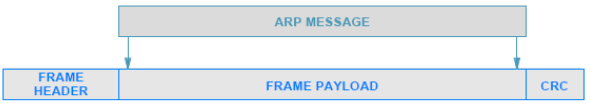
\includegraphics[width=\textwidth]{pic/arp_trans.png}
                    \label{Trama contenente il messaggio ARP}
                \end{figure}
                Quando viaggiano sulla rete fisica i messaggi ARP vengono rinchiusi in una trama, quindi il protocollo ARP viene considerato come dei dati trasportati dal Livello Data-Link.\\
                Nell'header della trama esiste un campo "\textit{type}" che indica il tipo di trama (per Ethernet il valore 0x806 denota i messaggi ARP). Il campo avrà lo stesso valore sia per le richieste che le risposte, andrà dunque controllato il valore del campo \textit{OPERATION} nel messaggio ARP.

        \subsection{Le Reti 802.11}
            \subsubsection{Architettura di riferimento delle WLAN}
                Con \textit{Station} (STA) si indica un terminale con capacità di accesso al messo wireless.\\
                Il \textit{Basic Service Set} (BSS) è l'insieme dei terminali che usano le stesse frequenze.\\
                Per \textit{Access Point} si intende una stazione integrata sia nella WLAN che nel "\textit{Distribution System}".\\
                Il \textit{Portal} è un Bridge verso le altre reti.\\
                Il \textit{Distribution System}, infine, è una rete di interconnessione per formare una unica rete logica partendo da diverse BSS.\\
                \\
                Nello specifico il BSS è formato da un insieme di terminali con lo stesso protocollo MAC che competono per l'accesso allo stesso mezzo condiviso. Questo può essere isolato o no, in questo caso esso sarebbe collegato ad un \textit{Distribution System} attraverso un \textit{Access Point} che funziona come un Bridge.

            \subsubsection{Il Livello MAC nelle reti 802.11}
                L'obiettivo è quello di modificare il CSMA al fine di evitare le collisioni, per questo è stato creato il \textbf{CSMA/CA} (Collision Avoidance).

                \paragraph{Distributed Coordination Function (DCF)} Basata sul CSMA/CA, utilizza un algoritmo per la risoluzioni delle contese, tramite questo è possibile dare accesso a tipi diversi di traffico. Il traffico ordinario si appoggia direttamente su DCF.
                \paragraph{Point Coordination Function (PCF)} Supporta il traffico Real-Time. Si basa sul "\textit{polling}" coordinato da un \textit{Centralized Point Coordinator}. PCF è costruito su DCF e sfrutta le sua funzionalità per dare accesso agli utenti.\\
                \\
                Entrambi possono funzionare contemporaneamente sulla stessa BSS, fornendo alternatamente periodi con e senza contesa. Dei due PCF è il meno usato.

            \subsubsection{Time Slots}
                Il tempo viene diviso in intervalli, chiamati \textit{Slot}, essi sono le unità di tempo del sistema e variano in base all'implementazione del Livello Fisico.\\
                Le stazioni si sincronizzano
                \begin{itemize}
                    \item nella modalità "\textit{infrastructure}, con l'\textit{Access Point}
                    \item nella modalità "\textit{ad hoc}, tra di loro
                \end{itemize}

                \subsubsubsection{Inter-Frame Space}
                Intervallo di tempo tra la trasmissione di trame, viene usato per stabilire dei livelli di priorità nell'accedere al canale. La durata dipende dall'implementazione fisica.

                Esistono 4 tipi di \textit{IFS}:
                \begin{itemize}
                    \item \textbf{SIFS}: Short IFS
                    \item \textbf{PIFS}: Point coordination IFS (> SIFS)
                    \item \textbf{DIFS}: Distributed IFS (> PIFS)
                    \item \textbf{EIFS}: Extended IFS (> DIFS)
                \end{itemize}

                \paragraph{Point coordination IFS}: Priorità media per servizi Real-Time che usano PCF. Il valore è dato da \textit{SIFS + 1 time-slot}. Usato dal controller centrale nel PCF durante il polling.
                \paragraph{Distributed IFS}: Priorità più bassa per il servizio di invio asincrono. Valore dato da \textit{SIFS + 2 time-slot}. Usato dalle trame per l'invio asincrono con ritardo minimo nel caso di contesa del canale.
                
            \subsubsection{DCF con CSMA/CA}
                Una stazione con dei dati da trasmettere ascolta in canale
                \begin{enumerate}
                    \item Se il canale è libero
                          \begin{itemize}
                              \item Continua ad ascoltare per capire se il mezzo rimane libero per un tempo pari a DIFS. I questo caso ai può trasmettere subito.
                          \end{itemize}
                    \item Se il canale è occupato
                          \begin{itemize}
                              \item La stazione continua a monitorare il mezzo fino a quando la trasmissione corrente è finita. Questo avviene sia perchè il mezzo risulta occupato fin dall'inizio sia perchè diventa occupato durante il DIFS.
                          \end{itemize}
                    \item Quando la trasmissione corrente è finita, la stazione aspetta un altro DIFS
                          \begin{itemize}
                              \item Se, dopo il DIFS, il canale è nuovamente occupato, si torna al punto 2
                          \end{itemize}
                    \item Se il mezzo rimane libero per un DIFS
                          \begin{itemize}
                              \item La stazione estrae un numero casuale di slot uniformemente distribuito all'interno di una \textbf{Contention Window} [0, CW-1]
                                    \begin{itemize}
                                        \item \textit{Contatore di Backoff}
                                    \end{itemize}
                              \item Finchè il canale resta libero, la stazione decrementa il contatore man mano che il tempo passa. Se questo arriva a 0 la stazione trasmette.                       
                          \end{itemize}
                    \item Se il canale torna ad essere occupato prima che il contatore arrivi a 0
                          \begin{itemize}
                              \item Il contatore viene congelato e si torna al punto 2. Al punto 4, però, non verrà estratto un nuovo contatore ma si continuerà con il valore congelato.
                          \end{itemize}
                \end{enumerate}
                Per quanto concerne il \textit{Contatore di Backoff}, esso è un intero che corrisponde al numero di time-slot.\\
                Di fatto è una variabile uniformemente distribuita nell'intervallo [0, CW-1], dove \textit{CW} è il valore della \textbf{Contention Window}, esso viene aggiornato ad ogni tentativo di trasmissione
                \begin{itemize}
                    \item $ i=1 $: $ CW_1 = CW_{min} $
                    \item $ i>1 $: $ CW_i = 2CW_{i-1} $ (per >1 si intende numero di tentativi consecutivi di trasmissione)
                    \item $ \forall i  $: $ CW_i \leq CW_{max} $ 
                \end{itemize}
                Ricapitolando, la prima stazione a cui scade il Contatore di Backoff inizia la trasmissione, le stazioni che percepiscono la trasmissione congelano il loro Backoff, che verrà fatto ripartire nel successivo periodo di contesa.\\
                \\
                In caso di collisione, la $ CW_{max} $ raddoppia, quindi la lunghezza del tempo di Backoff aumenta esponenzialmente in caso di collisioni consecutive.\\
                Si seleziona quindi un nuovo valore della CW randomicamente nell'intervallo [0, $ CW_{max} $]\\
                \\
                La stazione che riceve le trame manda un ACK immediatamente dopo la ricezione, senza ascoltare prima il mezzo (nella maggior parte delle implementazioni l'invio degli ACK è la sciato ai livelli superiori)
                
            \subsubsection{DCF con RTS/CTS}
                Introduciamo una serie di problematiche risolvibili con la metodologia \textit{RTS/CTS}

                \subsubsubsection{Problema del Terminale Nascosto}
                    Il segnale generato dalle stazioni (o dall'Access Point) è percepibile solo fino ad una certa distanza, questa dipende dalla potenza di emissione del segnale.\\
                    A causa di particolari disposizioni spaziali il segnale emesso da una stazione può essere percepito solo da un sottinsieme di stazioni. da qui nasce il \textit{Problema del Terminale Nascosto}.
                    \begin{figure}[H]
                        \centering
                        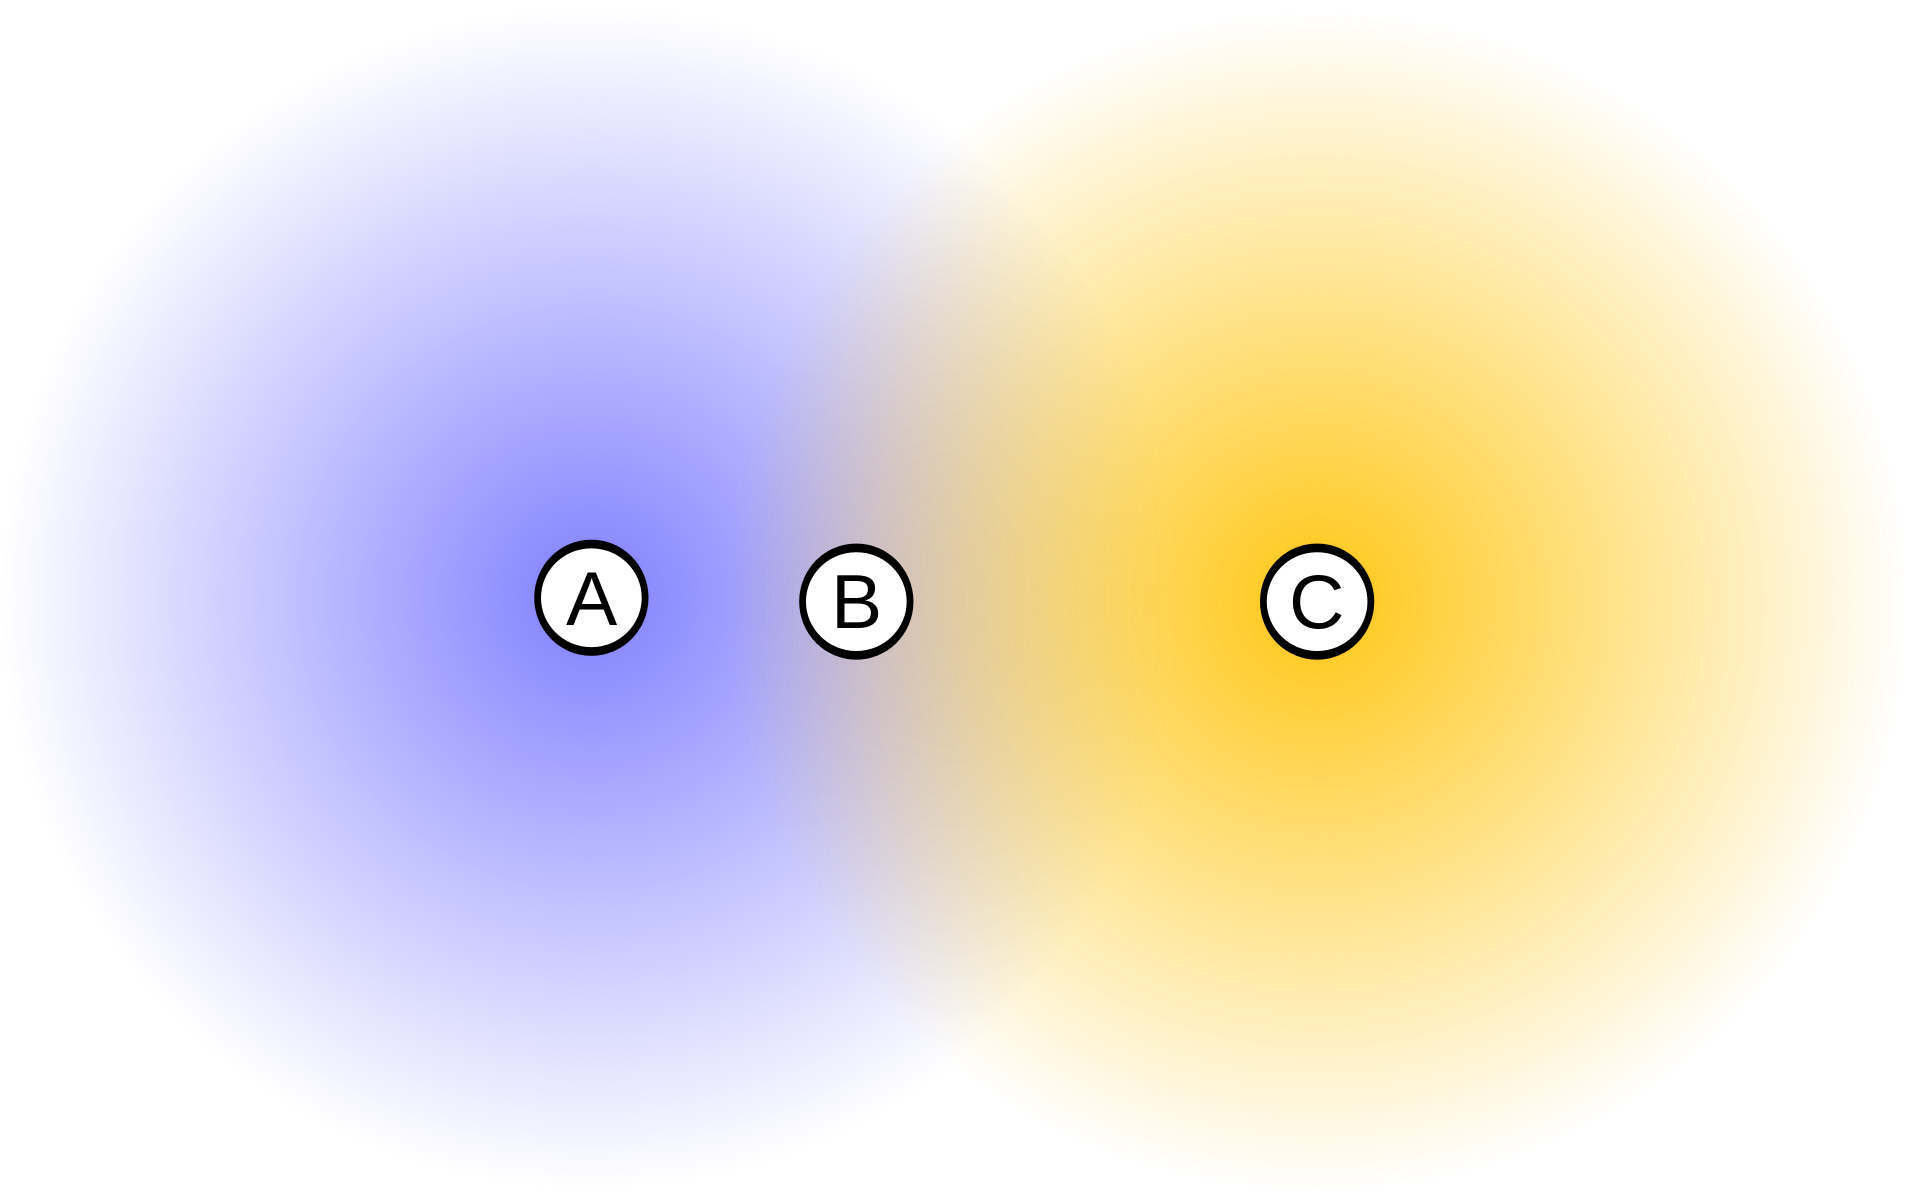
\includegraphics[width=\textwidth]{pic/terminale_nascosto.png}
                        \label{Problema del Termiale Nascosto}
                    \end{figure}
                    Descriviamo ora cosa succede precisamente
                    \begin{itemize}
                        \item A invia una trama a B
                        \item C ascolta il canale, non rilevando però la trasmissione di A (essendo fuori dal suo range, \textit{giallo} nel grafico)
                        \item Pensando che il canale sia libero, C invia una trama a B, causando una collisione
                    \end{itemize}

                \subsubsubsection{Problema del Terminale Esposto}
                    Sostanzialmente si tratta del problema opposto, una stazione non trasmette in quanto rileva una trasmissione tra altre due stazioni, che però non influenzerebbero la la sua.\\
                    Questo problema è dato dal posizionamento troppo ravvicinato delle stazioni nella sottorete.
                    \begin{figure}[H]
                        \centering
                        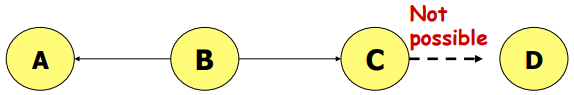
\includegraphics[width=\textwidth]{pic/terminale_esposto.png}
                        \label{Problema del Terminale Esposto}
                    \end{figure}
                    Più precisamente
                    \begin{itemize}
                        \item B invia delle trame ad A e C vuole inviarne a D
                        \item C ascolta il canale e rileva la trasmissione da B ad A
                        \item C non trasmette nonostante egli possa farlo, dato che non disturberebbe in alcun modo la trasmissione
                    \end{itemize}

                \subsubsubsection{RTS/CTS}
                    Con lo scopo di risolvere questi problemi sono stati introdotti \textit{RTS} e \textit{CTS}.
                    La sorgente, dopo aver percepito il canale libero per un intervallo di tempo pari a DIFS, invia una trama \textit{RTS}, a cui il ricevente risponderà con una trama \textit{CTS} dopo in intervallo SIFS. A questo punto i dati possono essere trasmessi.
                    Vediamo dunque, dopo questa introduzione, come vengono risolti i problemi del Terminale Nascosto ed Esposto

                    \paragraph{Problema del Terminale Nascosto}
                        \begin{itemize}
                            \item A invia una trama RTS a B
                            \item B invia, come risposta, una trama CTS in broadcast
                            \item A e C ricevono la trama CTS
                            \item C, sapendo che verranno inviati dei dati a B, evita di trasmettere
                            \item A può inviare dati a B senza preoccuparsi di possibili collisioni 
                        \end{itemize}
                        \begin{figure}[H]
                            \centering
                            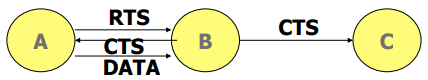
\includegraphics[width=\textwidth]{pic/nascosto_cts_rts.png}
                            \label{Soluzione al Terminale Nascosto con RTS/CTS}
                        \end{figure}
                        Al fine di mettere a conoscenza le altre stazioni del tempo per cui intende trasmettere, A include la lunghezza della trasmissione nella trama RTS. Quest'informazione verrà poi inclusa anche nella trama CTS da B, in modo che tutte le stazioni che riceveranno la CTS sapranno per quanto dovranno attendere. 

                    \paragraph{Problema del Terminale Esposto}
                        \begin{itemize}
                            \item B invia una trama RTS ad A, questa verrà dunque percepita anche da C
                            \item A risponde a B con una trama CTS, che non verrà però sentita da da C, in quanto fuori range
                            \item C assume quindi di non essere raggiungibile, quindi procede con la trasmissione a D
                        \end{itemize}
                        \begin{figure}[H]
                            \centering
                            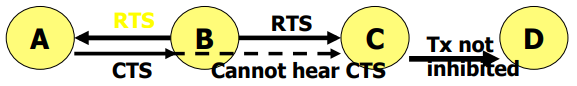
\includegraphics[width=\textwidth]{pic/esposto_cts_rst.png}
                            \label{Soluzione al Terminale Esposto con RTS/CTS}
                        \end{figure}

        \subsection{Network Allocation Vector}
            Nell'802.11 l'ascolto del canale è sia \textit{fisico} che "\textit{virtuale}". Se anche una sola delle due indica il canale come occupato, allora 802.11 lo considera tale.\\
            L'ascolto \textit{virtuale} è fornito dal \textbf{Network Allocation Vector (NAV)}.\\
            La maggior parte delle trame 802.11 includono un campo \textit{length} con la lunghezza della trama, i nodi che le percepiscono impostano quindi il NAV al tempo in cui si aspettano che il mezzo sia libero. Avendo NAV >0 il mezzo sarà considerato occupato.\\
            Non dovendo restare costantemente in ascolto le WLAN possono così risparmiare energia.

\end{document}
